% \documentclass[mat2, tisk]{fmfdelo}
% \documentclass[fin2, tisk]{fmfdelo}
\documentclass[isrm2, tisk]{fmfdelo}
% \documentclass[ped, tisk]{fmfdelo}
% Če pobrišete možnost tisk, bodo povezave obarvane,
% na začetku pa ne bo praznih strani po naslovu, …

%%%%%%%%%%%%%%%%%%%%%%%%%%%%%%%%%%%%%%%%%%%%%%%%%%%%%%%%%%%%%%%%%%%%%%%%%%%%%%%
% METAPODATKI
%%%%%%%%%%%%%%%%%%%%%%%%%%%%%%%%%%%%%%%%%%%%%%%%%%%%%%%%%%%%%%%%%%%%%%%%%%%%%%%

% LTeX: language=sl-SI

% - vaše ime
\avtor{Tim Kalan}

% - naslov dela v slovenščini
\naslov{Večstranski podpisi}

% - naslov dela v angleščini
\title{Multisignatures}

% - ime mentorja/mentorice s polnim nazivom:
%   - doc.~dr.~Ime Priimek
%   - izr.~prof.~dr.~Ime Priimek
%   - prof.~dr.~Ime Priimek
%   za druge variante uporabite ustrezne ukaze
\mentor{doc.~dr.~Tilen Marc}
% \somentor{...}
% \mentorica{...}
% \somentorica{...}
% \mentorja{...}{...}
% \somentorja{...}{...}
% \mentorici{...}{...}
% \somentorici{...}{...}

% - leto magisterija
\letnica{2025}

% - povzetek v slovenščini
%   V povzetku na kratko opišite vsebinske rezultate dela. Sem ne sodi razlaga
%   organizacije dela, torej v katerem razdelku je kaj, pač pa le opis vsebine.
\povzetek{Tukaj napišemo povzetek vsebine. Sem sodi razlaga vsebine in ne opis tega, kako je delo organizirano.}

% - povzetek v angleščini
\abstract{An abstract of the work is written here. This includes a short description of
the content and not the structure of your work.}

% - klasifikacijske oznake, ločene z vejicami
%   Oznake, ki opisujejo področje dela, so dostopne na strani https://www.ams.org/msc/
\klasifikacija{94A60, 11T71}

% - ključne besede, ki nastopajo v delu, ločene s \sep
\kljucnebesede{kriptografija\sep digitalni podpis\sep Schnorrov podpis\sep večstranski podpis}

% - angleški prevod ključnih besed
\keywords{cryptography\sep digital signature\sep Schnorr signature\sep multisignature} % angleški prevod ključnih besed

% - neobvezna zahvala
% \zahvala{
%   Neobvezno.
%   Zahvaljujem se \dots
% }

% - program dela, ki ga napiše mentor z osnovno literaturo
\programdela{
  Mentor naj napiše program dela skupaj z osnovno literaturo.
}

\osnovnaliteratura{
% Literatura mora biti tukaj posebej samostojno navedena (po pomembnosti) in ne
% le citirana. V tem razdelku literature ne oštevilčimo po svoje, ampak uporabljamo
% ukaz \vnosliterature, v katerega vpišemo citat
  \vnosliterature{micali2001asm}
  % \vnosliterature{gurtin1982introduction}
  % \vnosliterature{zienkiewicz2000finite}
  % \vnosliterature{STtemplate}
}

% - ime datoteke z viri (vključno s končnico .bib), če uporabljate BibTeX
\literatura{literatura.bib}

%%%%%%%%%%%%%%%%%%%%%%%%%%%%%%%%%%%%%%%%%%%%%%%%%%%%%%%%%%%%%%%%%%%%%%%%%%%%%%%
% DODATNE DEFINICIJE
%%%%%%%%%%%%%%%%%%%%%%%%%%%%%%%%%%%%%%%%%%%%%%%%%%%%%%%%%%%%%%%%%%%%%%%%%%%%%%%

% naložite dodatne pakete, ki jih potrebujete
\usepackage{units}        % fizikalne enote kot \unit[12]{kg} s polovico nedeljivega presledka, glej primer v kodi
\usepackage{graphicx}     % za slike
\usepackage{subcaption}
\usepackage{tikz}
\usetikzlibrary{shapes,calc,positioning,arrows,}

\pgfarrowsdeclarecombine{twotriang}{twotriang}%    double headed arrow
{stealth'}{stealth'}{stealth'}{stealth'} 

% VEČ ZANIMIVIH PAKETOV
% \usepackage{array}      % več možnosti za tabele
% \usepackage[list=true,listformat=simple]{subcaption}  % več kot ena slika na figure, omogoči slika 1a, slika 1b
% \usepackage[all]{xy}    % diagrami
% \usepackage{doi}        % za clickable DOI entrye v bibliografiji
% \usepackage{enumerate}     % več možnosti za sezname

% Za barvanje source kode
% \usepackage{minted}
% \renewcommand\listingscaption{Program}

% Za pisanje psevdokode
\usepackage{algpseudocode}  % za psevdokodo
\usepackage{algorithm}
\floatname{algorithm}{Algoritem}
\renewcommand{\listalgorithmname}{Kazalo algoritmov}

% deklarirajte vse matematične operatorje, da jih bo LaTeX pravilno stavil
% \DeclareMathOperator{\...}{...}

% vstavite svoje definicije ...
\newcommand{\R}{\mathbb R}
\newcommand{\N}{\mathbb N}
\newcommand{\Z}{\mathbb Z}
% Lahko se zgodi, da je ukaz \C definiral že paket hyperref,
% zato dobite napako: Command \C already defined.
% V tem primeru namesto ukaza \newcommand uporabite \renewcommand
\newcommand{\C}{\mathbb C}
\newcommand{\Q}{\mathbb Q}

\newcommand{\todo}[2][]{%
    \textcolor{red}{%
        \\ \textbf{\uppercase{todo: #2}}%
        \\%
        \ifx&#1&% Check if the optional parameter is empty
        \else%
            \textcolor{blue}{\uppercase{ideja:} #1}%
            \\%
        \fi%
    }%
}
%%%%%%%%%%%%%%%%%%%%%%%%%%%%%%%%%%%%%%%%%%%%%%%%%%%%%%%%%%%%%%%%%%%%%%%%%%%%%%%
% ZAČETEK VSEBINE
%%%%%%%%%%%%%%%%%%%%%%%%%%%%%%%%%%%%%%%%%%%%%%%%%%%%%%%%%%%%%%%%%%%%%%%%%%%%%%%

\begin{document}

\section{Uvod}
% Napišite kratek zgodovinski in matematični uvod.  Pojasnite motivacijo za problem, kje
% nastopa, kje vse je bil obravnavan. Na koncu opišite tudi organizacijo dela -- kaj je v
% katerem razdelku.
Odkar se je na svetu pojavil koncept (ročnega) podpisa, je večina primerov uporabe temeljila na
pridobivanju podpisov več deležnikov, saj je bila večina podpisanih dokumentov sporazum ali pogodba
med večimi deležniki. Odličen primer je npr.\ Deklaracija neodvisnosti Združenih držav
Amerike, vidna na sliki~\ref{fig:declaration}. 

\begin{figure}[ht]
  \centering
  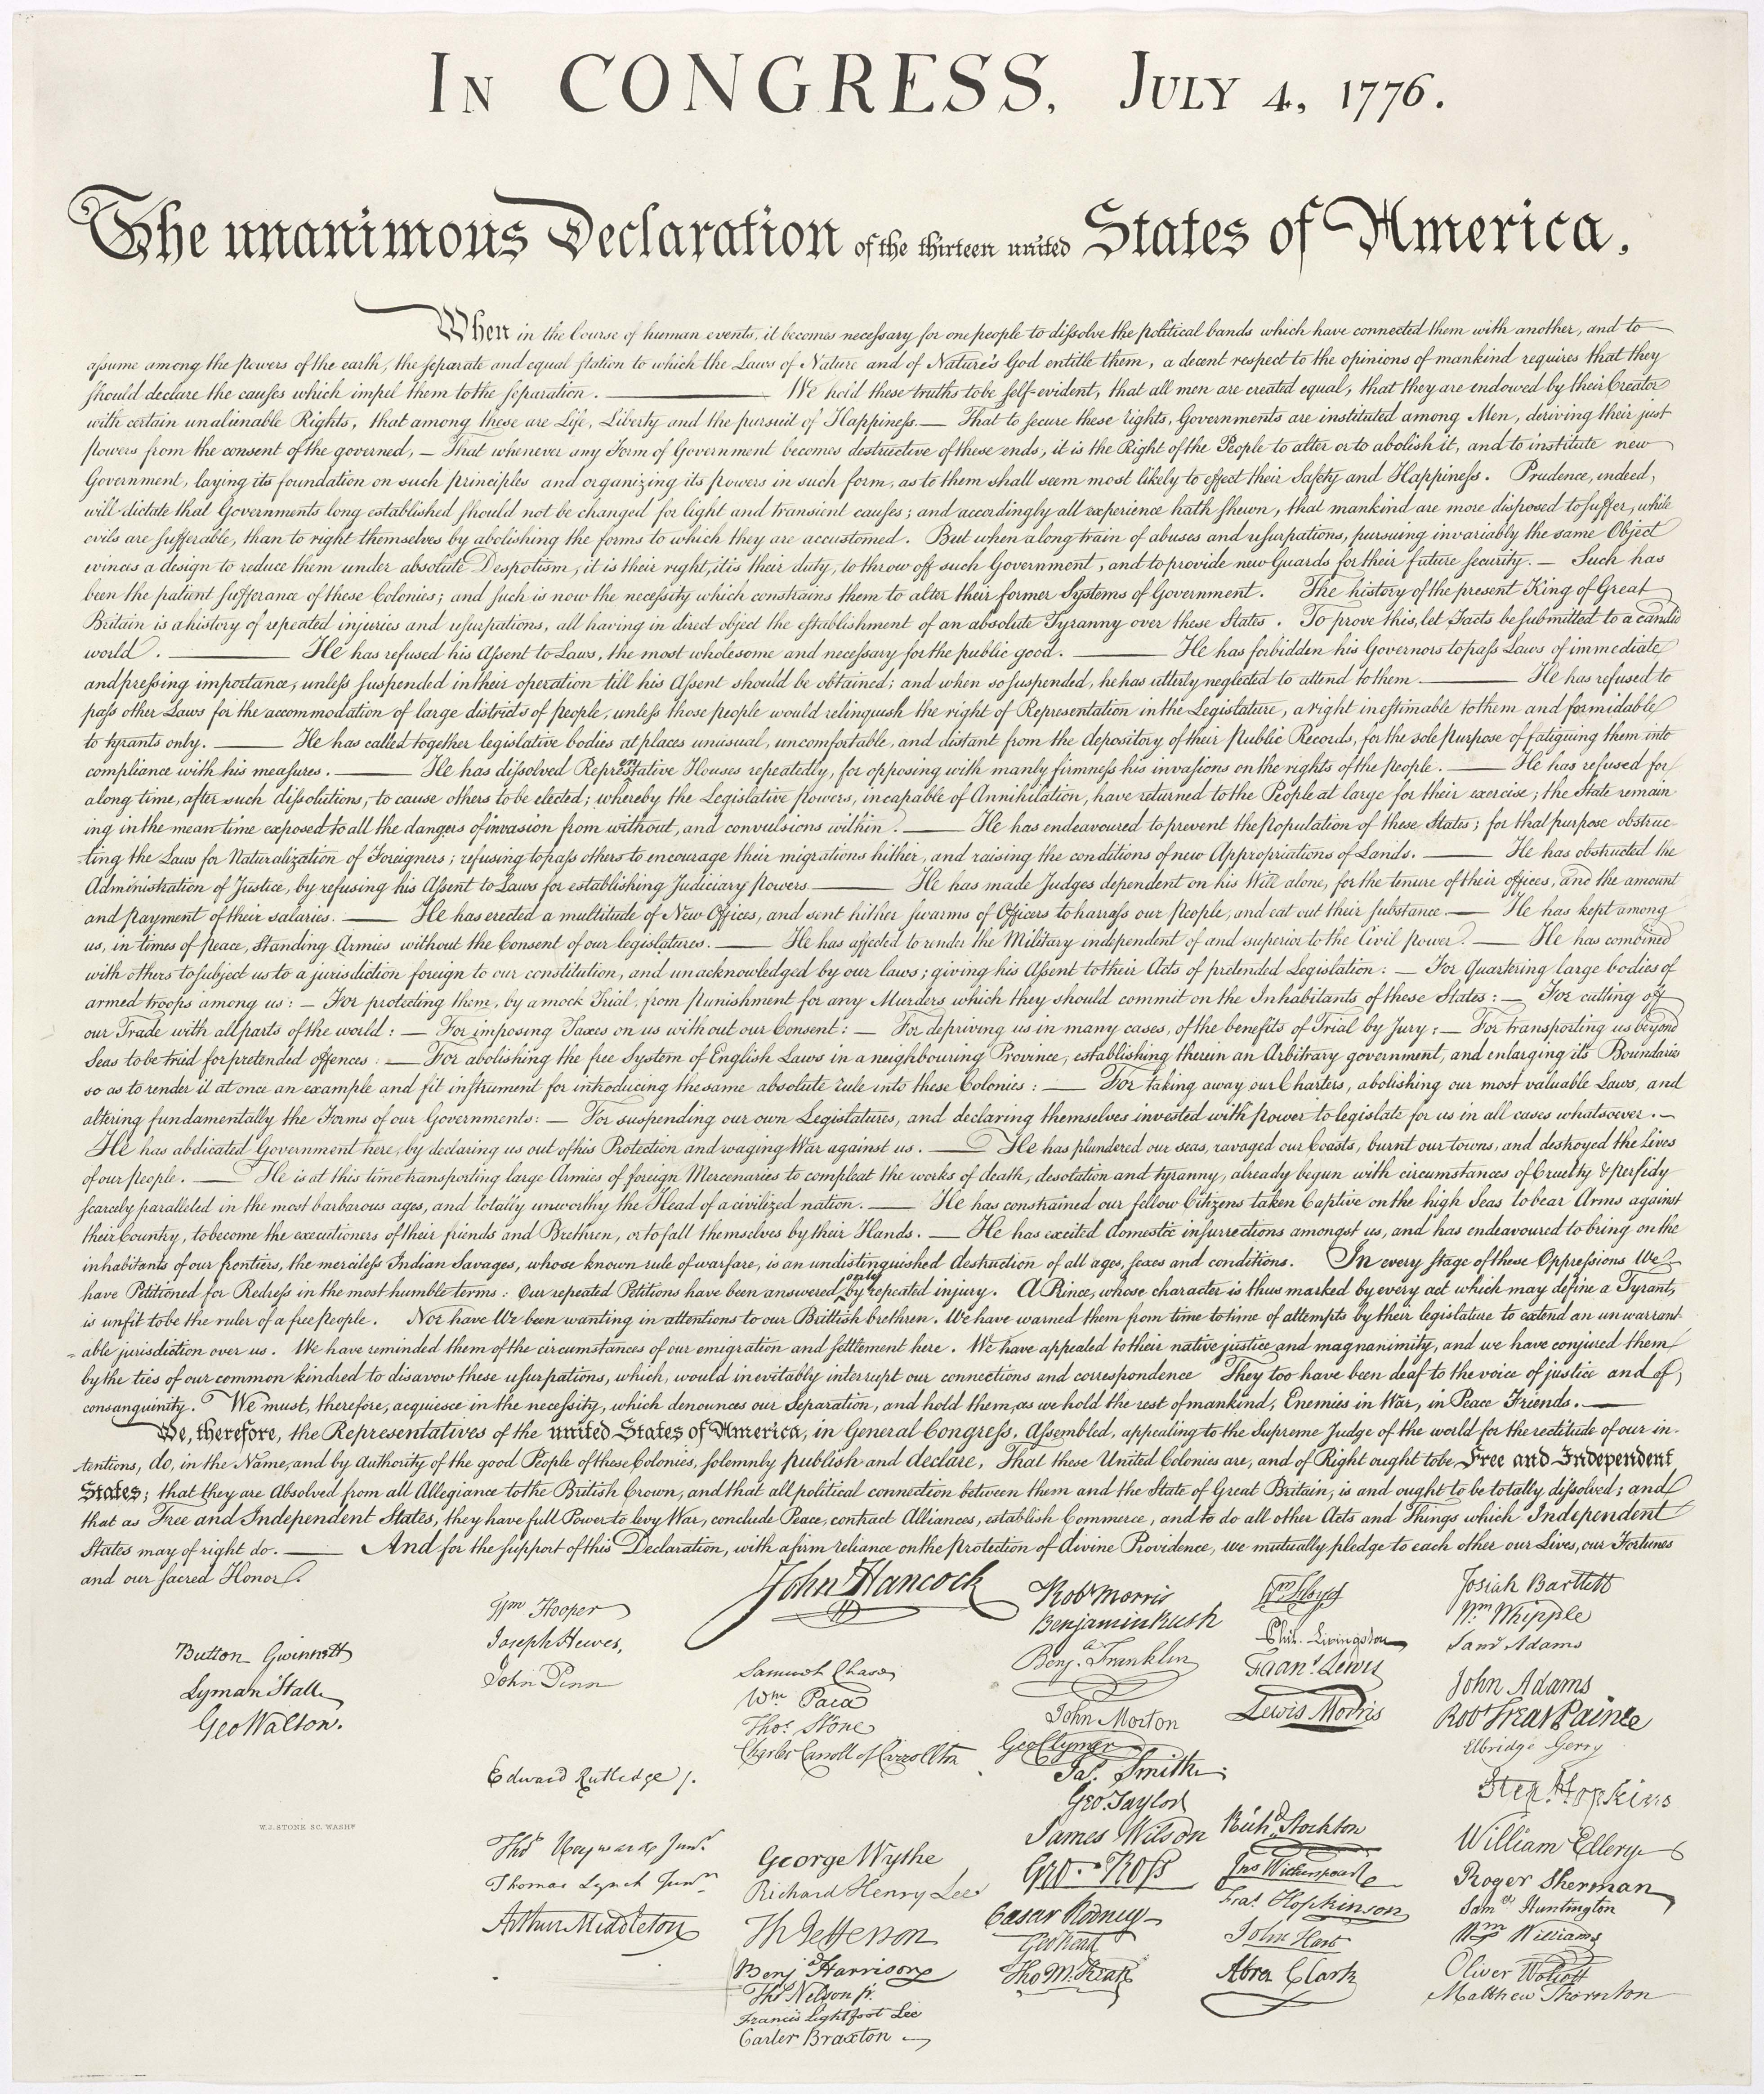
\includegraphics[width=0.5\textwidth]{images/declaration.jpg}
% \caption[caption za v kazalo]{Dolg caption pod sliko}
  \caption[Deklaracija neodvisnosti Združenih držav Amerike.]{Deklaracija neodvisnosti Združenih 
  držav Amerike s podpisi podpornikov spodaj. Vir slike Wikipedia~\cite{doi}.}
  \label{fig:declaration}
\end{figure}

S pojavom računalnika in napredkom v kriptografiji se je pojavila alternativna oblika podpisovanja.
\textit{Digitalni podpisi} so dandanes povsod. Uporabljeni so vsakič, ko dostopamo do spletnih
strani, prenašamo podatke ali pa opravljamo kakršnakoli plačila. Poleg avtomatiziranih podpisovanj,
ki se zgodijo v ozadju zgoraj omenjenih procesov, pa so digitalni podpisi na voljo tudi kot alternativa
ročnemu podpisu človeka. V praktično vseh pogledih so mnogo varnejši od tradicionalnih podpisov,
omogočajo bolj sistematično preverjanje (prek računalnikov) in so skorajda enostavnejši za uporabo
in prenašanje.

Prav tako lahko digitalne podpise uporabimo, če mora skupina deležnikov podpisati pogodbo -- vsak
enostavno pripne svoj digitalni podpis. Če je skupina velika, če je računska moč omejena
(npr.\ če želimo zmanjšati ceno transakcij pri tehnologiji veriženja blokov), ali pa če enostavno
želimo preverjevalcu podpisov olajšati delo, lahko poskrbimo, da se skupina podpiše z enim samim,
\textit{večstranskim} podpisom. Ta podpis vseeno priča o vseh podpisnikih, njegova verifikacija oz.\
preverjanje, pa zajema približno enako dela, kot preverjanje enega samega podpisa.

Taki podpisi so samo en izmed možnih načinov, kako se skupina podpiše. Od ostalih načinov izstopajo
po tem, da omogočajo vpogled v sestavo skupine podpisnikov, kar nudi preverjevalcu več informacij
pri odločanju, če je podpis sprejemljiv, hkrati pa ohranja odgovornost individualnih članov skupine.
Pri tradicionalnih skupinskih podpisih podpis samo priča o podpisu celotne skupine, ustvari pa ga
lahko katerkoli član. Take lastnosti so v določenih primerih zelo zaželene, npr.\ pri tehnologiji
veriženja blokov je zelo pomembno, da je znano iz katerih naslovov prihajajo transakcije. To, v
kombinaciji s popularizacijo Schnorrovega podpisa, je privedlo mnogo raziskovalcev do želje po
večstranskih podpisih, ki vrnejo navadne Schnorrove podpise, in so tako enostavno zamenljivi.

V poglavju~\ref{sec:osnove} najprej predstavimo kriptografske osnove, ki so potrebne za razumevanje besedila.
To zajema modularno aritmetiko in grupe, zgoščevalne funkcije, kriptografijo javnega ključa, nekaj
splošnih definicij pri digitalnih podpisih in potem še nekaj besed o varnosti. V poglavju~\ref{sec:schnorr}
predstavimo Schnorrov podpis, ki je osnova za ostale sheme, ki jih obravnavamo. V 
poglavju~\ref{sec:skpine} so predstavljeni vsi možni načini za podpisovanje skupin. Poglavje~\ref{sec:multischnorr}
predstavi večstranski Schnorrov podpis, tam tudi dokažemo njegovo varnost v modelu slučajnega oraklja.

\section{Kriptografske osnove}
\label{sec:osnove}
Preden si lahko natančneje pogledamo, kako lahko skupina generira en sam podpis sporočila, si moramo 
pogledati nekaj kriptografskih osnov. Bolj kompleksnejši pojmi bodo opisani sproti, namen tega 
poglavja je predstaviti stvari, ki so predpogoj za branje praktično kakršnegakoli kriptografskega 
besedila s področja digitalnih podpisov.

\subsection{Aritmetika v \texorpdfstring{$\Z_p^*$}{Zp∗}}
V kriptografiji imamo pogosto opravka z multiplikativnimi grupami, najenostavnejša med njimi (in 
tudi tradicionalno največ uporabljena) je \textit{multiplikativna grupa naravnih števil modulo $p$},
ki jo označimo $\Z_p^*$. Njeni elementi so števila v $\{0, 1, \dots, p - 1\}$, ki so tuja številu $p$.
V posebnem primeru, ko je $p$ praštevilo, so to torej števila \{1, 2, \dots, p - 1\} in je red grupe
(število elementov) $\text{ord}(\Z_p^*) = |\Z_p^*| = p - 1$. Operacija v tej grupi je, kot ime že
nakazuje, množenje modulo $p$.

Spomnimo se, da je red elementa $g$ v grupi najmanjše naravno število $q$, da velja $g^q \equiv 1 \pmod p$, 
kjer je $1$ enota za množenje. V primeru, da je $p$ praštevilo, je grupa $\Z_p^*$ \textit{ciklična},
kar pomeni, da v njej obstaja element $g$, katerega red je enak redu grupe, torej $\text{ord}(g) = p - 1$.
V tem primeru se $g$ imenuje \textit{generator}.

\begin{primer}[Grupa $\Z_{11}^*$]
\label{primer:Z11}
Ker je $11$ praštevilo, v grupi $\Z_{11}^*$ obstaja generator, oz.\ je grupa ciklična z redom $10 = 
11 - 1$. Z zaporednim računanjem potenc lahko vidimo, da je $\text{ord}(2) = 10$, torej je $2$ 
generator.

\begin{minipage}{0.45\textwidth}
    \begin{align*}
        2^1 &\equiv 2 \pmod{11} \\
        2^2 &\equiv 4 \pmod{11} \\
        2^3 &\equiv 8 \pmod{11} \\
        2^4 &\equiv 5 \pmod{11} \\
        2^5 &\equiv 10 \pmod{11} 
    \end{align*}
\end{minipage}
\begin{minipage}{0.45\textwidth}
    \begin{align*}
        2^6 &\equiv 9 \pmod{11} \\
        2^7 &\equiv 7 \pmod{11} \\
        2^8 &\equiv 3 \pmod{11} \\
        2^9 &\equiv 6 \pmod{11} \\
        2^{10} &\equiv 1 \pmod{11} 
    \end{align*}
\end{minipage}

\end{primer}

\begin{opomba}
    Spomnimo se \textit{kongruence}: $a \equiv b \pmod m \iff m \text{ }|\text{ } a - b$.
\end{opomba}

Za konec tega popdpoglavja si oglejmo še dve trditvi, ki bosta pomembni pri dokazovanju pravilnega
delovanja Schnorrovega podpisa.

\begin{trditev}
\label{trd:mod-q}
    Naj bosta $p$ in $q$ praštevili, kjer $q$ deli $p - 1$, oz.\ $q \text{ }|\text{ } p - 1$. Naj
    bo $g$ element grupe $\Z_p^*$ reda $q$, kar pomeni, da je $g^q \equiv 1 \pmod p$. Naj bo $k$
    naravno število. Potem velja 
    $$ 
    g^k \bmod p = g^{k \bmod q} \bmod p.
    $$
\end{trditev}
\begin{dokaz}
    Po osnovnem izreku o deljenju naravnih števil, lahko $k$ na en sam način zapišemo kot $k = nq + r$, 
    kjer velja $n \in \N, r < q$.

    Leva stran enačbe se potem prepiše 
    \begin{align*}
        g^k \bmod p &= g^{nq + r} \bmod p = \\ 
                    &= (g^q)^n g^r \bmod p = \\ 
                    &= 1^n g^r \bmod p = \\ 
                    &= g^r \bmod p.
    \end{align*}
    Desna stran pa se prepiše kot 
    \begin{align*}
        g^{k \bmod q} \bmod p &= g^{(nq + r) \bmod q} \bmod p = \\ 
                              &= g^r \bmod p.
    \end{align*}
    Ker sta obe strani enaki, je trditev dokazana.
\end{dokaz}

\begin{trditev}
\label{trd:mod-mn-pt}
    Naj bodo $a$, $b$ in $p$ naravna števila. Potem za modularno množenje in potenciranje velja
    \begin{align}
        a \cdot b \bmod p &= (a \bmod p) \cdot (b \bmod p) \bmod p, \label{eq:mod-prod} \\
        a^b \bmod p &= (a \bmod p)^b \bmod p. \label{eq:mod-exp} 
    \end{align}
\end{trditev}
\begin{dokaz}
    $a$ in $b$ lahko po osnovnem izreku o deljenju naravnih števil na en sam način zapišemo kot 
    \begin{align*}
        a &= n_a p + r_a, \\
        b &= n_b p + r_a,
    \end{align*}
    kjer velja $r_a < p$.

    \eqref{eq:mod-prod}: Levo stran preoblikujemo
    \begin{align*}
        a \cdot b \bmod p &= (n_a p + r_a) \cdot (n_b p + r_b) \bmod p = \\
                          &= (n_a n_b p^2 + n_a p r_b + n_b p r_a + r_a r_b) \bmod p = \\
                          &= r_a r_b \bmod p,
    \end{align*}
    desno pa
    \begin{align*}
        (a \bmod p) \cdot (b \bmod p) \bmod p &= (n_a p + r_a \bmod p) \cdot (n_b p + r_b \bmod p) \bmod p = \\
                          &= r_a r_b \bmod p.
    \end{align*}
    Ker se strani ujemata, je trditev dokazana.

    \eqref{eq:mod-exp}: Ker je potenciranje samo zaporedna uporaba množenj, lahko trditev pokažemo z 
    indukcijo na $b$ in enačbo~\eqref{eq:mod-prod}:
    \begin{itemize}
        \item $b = 2$: Primer, ko je $b = 1$ (ali $b = 0$) je trivialen, če pa je $b = 2$, pa se 
            problem reducira v 
            $$ 
            a \cdot a \bmod p \stackrel{?}{=} (a \bmod p) \cdot (a \bmod p) \bmod p,
            $$
            kar drži neposredno po enačbi~\eqref{eq:mod-prod}.
        \item $n \rightarrow n + 1$: Predpostavimo, da enačba~\eqref{eq:mod-exp} drži za $b = n$ (I.P.). 
            Ko je $b = n + 1$, dobimo 
            \begin{align*}
                a^{n + 1} \bmod p &= a^n a \bmod p = \\ 
                                  &\stackrel{\eqref{eq:mod-prod}}{=} (a^n \bmod p) (a \bmod p) \bmod p = \\
                                  &\stackrel{\text{I.P.}}{=} (a \bmod p)^n (a \bmod p) \bmod p = \\
                                  &= (a \bmod p)^{n + 1} \bmod p.
            \end{align*}
    \end{itemize}
    S tem je indukcija končana in trditev dokazana.
\end{dokaz}

\subsection{Zgoščevalne funkcije}
V grobem so (kriptografske) \textit{zgoščevalne funkcije} take funkcije, ki prejmejo poljubno dolg binarni 
niz (ki lahko predstavlja besede, številke, celotne dokumente, \dots), vrnejo pa binarni niz, ki ima
vnaprej določeno dolžino. Tem rezultatom pravimo \textit{zgostitve}. Namen zgoščevalnih funkcij je 
za dokument ustvariti unikaten niz, ki zelo verjetno unikatno identificira dokument. Želimo si, da
je v praksi nemogoče najti dva različna niza z enako zgostitvijo, natančno pa zgoščevalne funkcije
definiramo:

\begin{definicija} 
\label{def:hash}
    \textbf{Kriptografska zgoščevalna funkcija} $H: \{0, 1\}^* \rightarrow \{0, 1\}^n$ je funkcija, 
    ki slika binarne nize $m$ poljubne dolžine v njihove \textbf{zgostitve} $H(m)$, tj.\ binarne nize 
    vnaprej določene dolžine $n$. Zadoščati mora naslednjim lastnostim:
    \begin{itemize}
        \item \textbf{Določenost} pomeni, da bo zgoščevanje enakih nizov vedno privedlo do enake 
            zgostitve. Zapišemo lahko $\forall m: ((h_1 = H(m) \wedge h_2 = H(m)) \implies h_1 = h_2)$.
        \item \textbf{Učinkovitost} pomeni, da lahko računalnik izračuna poljubno zgostitev v doglednem 
            času. Izračun zgostitve mora biti računsko učinkovit. Ponavadi tu zahtevamo, da je časovna
            zahtevnost funkcije $H$ polinomska v dolžini vhodnega niza.
        \item \textbf{Enosmernost} oz.\ \textbf{odpornost na prasliko} pomeni, da iz predložene 
            zgostitve zelo težko ugotovimo, kateri niz je funkcija prejela kot vhod. Če torej poznamo 
            zgostitev $h$ za nek neznan $m$, je računsko neizvedljivo najti niz $m$, da velja $h = H(m)$.
        \item \textbf{Odpornost na drugo prasliko} pomeni, da če poznamo niz in njegovo zgostitev, 
            zelo težko najdemo drug niz z enako zgostitvijo. Če torej poznamo niz $m_1$, je računsko 
            neizvedljivo najti zgostitev $m_2$, da velja $H(m_1) = H(m_2)$.
        \item \textbf{Skoraj brez trčenj} oz.\ \textbf{odpornost na trčenja} pomeni, da je verjetnost,
            da imata dva izraza enako zgostitev, majhna. Želimo, da je računsko neizvedljivo
            najti dva niza  $m_1$ in $m_2$, ki imata enako zgostitev, oz.\ da velja $H(m_1) = H(m_2)$.
        \item \textbf{Učinek plazu} pomeni, da vsaka sprememba v vhodnem nizu povzroči veliko spremembo 
            v zgostitvi. Ob katerikoli spremembi se vsak bit zgostitve se spremeni z verjetnostjo 
            vsaj $1/2$.
    \end{itemize}
\end{definicija}

\begin{opomba}
    Vse varne kriptografske zgoščevalne funkcije, ki so v uporabi zadoščajo zgornjim lastnostim. To
    pomeni, da za nobeno od teh funkcij nihče še ni našel trka.
\end{opomba}

\begin{primer}
    Ena izmed najbolj znanih zgoščevalnih funkcij je \texttt{SHA-256}. Njeno ime pomeni \textit{Secure 
    Hash Algorithm} (slov.\ varen zgoščevalni algoritem), $256$ pa predstavlja dolžino vrnjene zgostitve. 
    Pogostokrat to ime zasledimo pri nameščanju programske opreme, kjer služi kot avtentikator, da smo res 
    naložili pravo stvar. Preverja namreč, da se zgostitvi naloženih in prenešenih datotek ujemajo.

    Za primer si lahko ogledamo zgostitvi dveh podobnih nizov, \textit{Ljubljana} in \textit{Ljubljena}. 
    Kljub podobnosti bomo videli, da sta rezultata popolnoma drugačna, kar si tudi želimo pri zgoščevalnih 
    funkcijah.
    \begin{verbatim}
    SHA-256(Ljubljana) =
    b7f147d8b4a6703a951336654355071f9752385f85d0860379e99b484aee7a82

    SHA-256(Ljubljena) =
    995d2d8ffb40e1838219e65dd2c665701ba34a90e11f7195a4b791838b6787fe
    \end{verbatim}
    Za preglednost nismo prevajali besed v binarne nize, to bi storili npr.\ z \texttt{ASCII} ali \texttt{UTF-8}
    tabelo. Prav tako smo rezultat napisali v šestnajstiškem sistemu, saj je tako krajši. Iz rezultatov
    pa nazorno vidimo učinek plazu, saj sta popolnoma drugačna.
\end{primer}

\subsection{Kriptografija javnega ključa}
Prve šifre, ki smo jih uporabljali ljudje, so bile \textit{simetrične}, kar pomeni, da sta osebi 
za komunikacijo obe morali poznati skriven \textit{ključ}, ki je definiral, kako je bila šifra 
ustvarjena. 

\begin{primer}[Cezarjeva šifra]
    Ena najbolj znanih šifer, ki izvira iz Antičnega Rima, je \textit{Cezarjeva šifra}. Njen ključ 
    je število, ki je krajše od dolžine naše abecede, v Cezarjevem primeru je bilo to število $3$.
    Šifra potem deluje tako, da vsako črko zamakne za toliko mest v abecedi, kolikor definira 
    ključ. Npr.\ za slovensko abecedo, bi šifra zamaknila črke:
    \begin{verbatim}
        A B C Č D E F G H I J K L M N O P R S Š T U V Z Ž
        Č D E F G H I J K L M N O P R S Š T U V Z Ž A B C
    \end{verbatim}
    To bi izraz \texttt{JAVNI KLJUČ} preslikalo v \texttt{MČARL NOMŽF}. Cezarjeva šifra se imenuje 
    tudi \textit{zamična šifra}.
\end{primer}

V prejšnjem stoletju pa se je pojavila alternativa, imenovana \textit{asimetrična kriptografija}, oz.\
\textit{kriptografija javnega ključa}. Glavna prednost te je, da osebi za komunikacijo ne rabita 
poznati enakega skrivnega ključa, vendar ima vsak od njiju par ključev, ki ju imenujemo \textbf{javni 
ključ} (angl.\ \textit{public key}) in \textbf{zasebni ključ} (angl.\ \textit{secret/private key}) in 
označimo kot par $(\text{pk}, \text{sk})$. Vsaka oseba objavi svoj javni ključ in poskrbi, da nihče 
ne izve, kaj je njen zasebni ključ. 

Šifriranje potem poteka tako, da pridobimo javni ključ od osebe, s katero želi komunicirati, ga uporabimo
za šifriranje in objavimo šifrirano sporočilo. Lastnik ustreznega zasebnega ključa (vsakemu javnemu pripada 
natanko en zasebni) potem pridobi šifrirano sporočilo in ga z zasebnim ključem dešifrira. Kriptosistemi
delujejo na način, da lahko sporočilo, šifrirano z javnim ključem dešifrira samo ustrezen zasebni ključ.
Tako zagotovimo varno komunikacijo. 

\begin{primer}[RSA]
\label{primer:rsa}
    En prvih algoritmov javnega ključa, ki se uporablja še danes, je \textit{RSA}. Njegova varnost izhaja 
    iz (domnevne) težavnosti problema iskanja prafaktorjev velikega števila. Svoj ključ definiramo tako, 
    da si izberemo dve (zelo veliki) praštevili $p$ in $q$, ter ju zmnožimo v $n = pq$. Za primer vzemimo 
    $p = 23$ in  $q = 17$. $n$ je potem enak $391$. Izbrati si moramo še eksponent $e$, vzemimo npr. $e = 3$. 
    Naš javni ključ je potem par 
    $$ 
    (n, e) = (391, 3).
    $$
    Postopek šifriranja poteka tako, da oseba, s katero komuniciramo, izbere sporočilo $m$, npr.\ 
    $m = 10$, pridobi naš javni ključ, in izračuna šifro $c$ kot
    $$
    c = m^e \bmod{n} = 10^3 \bmod{n} = 218.
    $$
    Dogovoriti se moramo še o zasebnem ključu. Za to bomo potrebovali eksponent za dešifriranje $d$,
    tako da bo veljalo 
    $$
    (m^e)^d \equiv 1 \pmod{\varphi(n)},
    $$ 
    kjer $\varphi$ označuje Eulerjevo funkcijo. Iščemo torej multiplikativni inverz eksponenta 
    $e$, modulo $\varphi(n)$. V našem primeru je to $d = 235$. Zasebni ključ je potem 
    $$ 
    (p, q, d) = (23, 17, 235). 
    $$
    Iz zasebnega ključa torej lahko kadarkoli izračunamo javnega, saj enostavno zmnožimo $p$ in $q$ 
    ter izračunamo inverz, v splošnem pa iz $n$ učinkovito ne moremo pridobiti faktorjev $p$ in $q$,
    kar nam zagotavlja varnost.

    Ko prejmemo šifrirano sporočilo $c$, ga dešifriramo tako, da izračunamo
    $$
    m = c^d \bmod{n} = 218^{235} \bmod{391} = 10.   
    $$
\end{primer}

Poleg šifriranja, brez da bi si delili ključ, pa je kriptografija javnega ključa omogočila tudi 
\textit{digitalne podpise}. Ti so uporabljeni vsakič, ko pošljemo transakcijo ali dostopamo do katerekoli 
spletne strani. Delujejo na podoben način, kot šifriranje z javnim ključem, le da najprej uporabimo 
zasebni ključ na sporočilu, prek javnega ključa pa preverjamo veljavnost podpisa. Velikokrat sta šifrianje 
in podpisovanje uporabljena hkrati, saj tako pošljemo šifrirano sporočilo, za katerega lahko oseba,
s katero komuniciramo preveri, da je res prišlo od nas.

\subsection{Digitalni podpisi}
Ideja \textit{kriptografskih} ali \textit{digitalnih podpisov} (angl.\ \textit{digital signatures}) je, 
da služijo kot izboljšava človeškega ročnega podpisa. Za razliko od ročnega podpisa, lahko z digitalnim 
dosežemo pravo identifikacijo posameznika, ki temelji na njegovem zasebnem ključu. Tako smo lahko 
za digitalno podpisan dokument prepričani, da ga je res podpisal lastnik točno določenega zasebnega ključa
(če predpostavimo, da podpisnik ključa ni posredoval nikomur). 

Podpis dokumenta poteka nekoliko drugače, kot pri ročnih podpisih. Pri ročnem podpisu ta postane del 
dokumenta, digitalni podpis pa je od njega ločen, vseeno pa nastane s pomočjo zgostitve podpisanega 
dokumenta, zato bo podpis za dva različna dokumenta vedno drugačen.

Ostane še vprašanje preverjanja avtentičnosti podpisa. Pri ročnem podpisu to lahko storimo prek 
primerjave z znanim, preverjeno avtentičnim podpisom. Ta postopek je zamuden in nenatančen, veliko 
večino ročnih podpisov je moč ponarediti z nekaj prakse. Preverjanje digitalnega podpisa pa temelji 
na kriptografiji javnega ključa. Ker je podpis nastal s pomočjo podpisnikovega zasebnega ključa,
lahko s pomočjo ujemajočega javnega ključa preverimo avtentičnost.

\begin{definicija}
\label{def:digisig}
    \textbf{Digitalni} ali \textbf{kriptografski podpis} $\mathcal{S} = (\mathcal{P}, \mathcal{G},
    \mathcal{S}, \mathcal{V})$ je četvorka učinkovitih algoritmov $\mathcal{P}$ za ustvarjanje parametrov
    podpisa, $\mathcal{G}$ za ustvarjanje ključa, $\mathcal{S}$ za podpisovanje in $\mathcal{V}$ za
    preverjanje podpisa. Definirana je nad končno množico možnih  sporočil $\mathcal{M}$, vrnjeni
    podpis pa leži v končni množici podpisov $\Sigma$.
    \begin{itemize}
        \item $\mathcal{P}$ je algoritem za ustvarjanje javnih parametrov podpisa. Definira grupo $G$,
            ki bo uporabljena pri podpisu. V praksi je ta korak izpuščen, sodelujoči pri podpisu
            uporabijo dobro poznane varne grupe. Formalno pa je to algoritem, ki prejme varnostni
            parameter $\lambda$ in vrne parametre grupe $G$, oz.\
            $$
            G = \mathcal{P}(\lambda).
            $$
        \item $\mathcal{G}$ je naključnostni algoritem za ustvarjanje para ključev $(\text{pk}, \text{sk})$, 
            ki za svoj vhod prejme parametre grupe $G$ (javno dostopni ali pa ustvarjeni prek $\mathcal{P}$).
            Z javnim ključem $\text{pk}$ lahko preverjevalec preveri avtentičnost podpisa, z zasebnim
            ključem $\text{sk}$ pa podpisnik podpisuje. Formalno velja
            $$
            (\text{pk}, \text{sk}) = \mathcal{G}(G).
            $$
        \item $\mathcal{S}$ je naključnostni algoritem, ki za svoja argumenta prejme zasebni ključ $\text{sk}$ 
            in sporočilo $m$, vrne pa podpis $\sigma$ sporočila $m$ z zasebnim ključem $\text{sk}$
            oz.\ 
            $$ 
            \sigma = \mathcal{S}(\text{sk}, m).
            $$
        \item $\mathcal{V}$ je determinističen algoritem, ki preverja veljavnost podpisov. Za svoje argumente
            prejme javni ključ $\text{pk}$, sporočilo $m$ in podpis $\sigma$, vrne $veljaven$, če je podpis 
            veljaven in $neveljaven$, sicer. Velja torej
            $$ 
            \mathcal{V}(\text{pk}, m, \sigma) = 
            \begin{cases}
                veljaven, & \sigma = \mathcal{S}(\text{sk}, m), \\
                neveljaven, & \sigma \neq \mathcal{S}(\text{sk}, m).
            \end{cases}
            $$
    \end{itemize}
\end{definicija}

\subsection{Interaktivni protokoli}
\todo{si interaktivni protokoli, identifikacijske in avtentikacijske sheme, dokazi (znanja) brez 
razkritja znanja, fiat-shamirjeva hevristika zasluži obravnavo posebaj?}

\subsection{Varnost}
Poglavitna lastnost vsakega kriptosistema je njegova \textit{varnost}. Ker je namen digitalnih podpisov
zagotoviti sogovorniku, da je sporočilo res poslal lastnik zasebnega ključa, je največja varnostna
skrb, da bi \textit{napadalec} lahko ponaredil pošiljateljev podpis in si s tem prisvojil njegovo 
identiteto. To napadalcu lahko uspe na več nivojih, od najmanj do najbolj škodljivega:

\begin{itemize}
    \item \textbf{Eksistencialno ponarejanje} (angl.\ \textit{existential forgery}) pomeni, da obstaja
        sporočilo, za katerega napadalec lahko ustvari ponarejen podpis (torej podpis, pri katerem
        ni bil uporabljen zasebni ključ). To pomeni, da lahko najde vsaj en par sporočila in podpisa
        $(m, \sigma)$, da velja $\mathcal{V}(\text{pk}, m, \sigma) = veljaven$.
    \item \textbf{Selektivno ponarejanje} (angl.\ \textit{selective forgery}) pomeni, da lahko napadalec 
        z nezanemarljivo verjetnostjo podpiše sporočilo, ki mu ga da nekdo drug in ga lastnik zasebnega
        ključa še ni podpisal. Torej, če napadalcu nekdo predloži sporočilo $m$, lahko z nezanemarljivo 
        verjetnostjo najde podpis $\sigma$, da velja $\mathcal{V}(\text{pk}, m, \sigma) = veljaven$.
    \item \textbf{Popoln zlom} (angl.\ \textit{total break}) pomeni, da napadalec pridobi 
        zasebni ključ napadenega in s tem pridobi vse potrebne podatke za podpisovanje poljubnih
        sporočil v njegovem imenu.
\end{itemize}

Poleg zgoraj definiranih \textit{ciljev napadalca}, lahko za vsak kriptosistem definiramo tudi
\textit{model napada}, in pa \textit{tip varnosti}, ki ga zagotavlja shema. Varnost večine shem za 
digitalne podpise temelji na (domnevni) težavnosti določenih matematičnih problemov.

Stinson~\cite{stinson2023crypto} definira naslednje modele napada:
\begin{itemize}
    \item \textbf{Napad samo s ključem} je napad, kjer napadalec pozna javni ključ žrtve $\text{pk}$. 
        Predpostavimo tudi, da napadalec vedno pozna delovanje sheme za podpisovanje $\mathcal{S}$
        in ima dostop do javnih parametrov podpisa $G$. Z javnim ključem torej lahko preverja
        veljavnost podpisov, ni pa prejel nobenega podpisanega sporočila.
    \item \textbf{Napad z znanimi sporočili} je napad, kjer napadalec poseduje seznam parov sporočil 
        in njihovih podpisov $(m_1, \sigma_1), (m_2, \sigma_2), \dots$, kjer za vsak $i$ velja 
        $\sigma_i = \mathcal{S}(\text{sk}, m_i)$.
    \item \textbf{Napad z izbranimi sporočili} je napad, kjer napadalec podpisniku da seznam sporočil $m_1,
        m_2, \dots$, ta pa mu vrne seznam podpisov, da za vsak $i$ velja $\sigma_i = \mathcal{S}(\text{sk}, 
        m_i)$. Napadalčev cilj je iz predloženih parov izvleči zasebni ključ, ali pa na nek drug način
        podpisati še ne podpisano sporočilo.
\end{itemize}

Ostane nam še pregled varnosti, ki jo lahko pričakujemo oz.\ zahtevamo od sheme za podpisovanje. 
Takšna shema ne more biti \textit{brezpogojno varna}, kar bi pomenilo, da je tudi z neomejenimi 
računskimi zmožnostmi nemogoče ponarediti podpis. To je zato, ker lahko napadalec sistematično 
preveri vse podpise za neko sporočilo s pomočjo algoritma $\mathcal{V}$, dokler ne najde pravega. 
Pričakujemo pa lahko \textit{računsko varnost}, kar pomeni, da napadalec ne more najti ponaredka 
v doglednem času, če ima omejene računske sposobnosti, in/ali pa \textit{dokazljivo varnost}, kar 
pomeni, da lahko varnost prevedemo na težavnost nekega matematičnega problema.

\subsubsection{Temelji varnosti}
V primeru~\ref{primer:rsa} smo omenili, da je varnost algoritma RSA odvisna od težavnosti problema
iskanja prafaktorjev velikega števila. To je le eden izmed mnogih problemov, ki služijo kot osnova
za varnost kriptografskih sistemov. V kriptografiji javnega ključa se pogosto srečamo s cikličnimi
grupami, ki podpirajo množenje. V nadaljevanju bomo pogosto uporabili operacijo množenja, za izračune
tipa 
$$
I = g^s,
$$
kjer je $g$ generator ciklične grupe, $s$ pa zasebni ključ. Zaradi notacije bi morda kdo hitro pomislil,
da lahko zgornjo enačbo obrnemo in $s$ izračunamo kot 
$$ 
s = \log_g(I).
$$
Taki izračuni v (nekaterih) cikličnih grupah žal (ali pa na srečo) niso tako enostavni, prišli smo do
koncepta \textit{diskretnega logaritma}. V diskretnih cikličih grupah, kot je npr.\ $\Z_p^*$, ni koncepta
urejenosti, kar smo videli tudi v primeru~\ref{primer:Z11}, zato nam ">približki"< logaritma ne pomagajo
čisto nič. Za izračun takih logaritmov se moramo zanesti na drugačne metode, kot za izračun navadnih.

\begin{definicija}[Problem diskretnega logaritma~\cite{boneh2023appcry}]
\label{def:dl}
    Naj bo $G$ ciklična grupa reda $q$, ki jo generira element $g$. Naj bo $h$ naključni element iz 
    grupe $G$. Naj velja $g^x = h$. Eksponent $x$ Potem imenujemo \textbf{Diskretni logaritem (DL)}.

    Zamislimo si igro, kjer izzivalec in nasprotnik kot vhod prejmeta opis grupe $G$ (torej $q$ in 
    $g \in G$). Izzivalec potem izbere naključen element $\alpha \in G$ in izračuna $h = g^{\alpha}$.
    $h$ pošlje nasprotniku, ta pa mora odgovoriti nazaj z elementom $\alpha$. To igro imenujemo 
    \textbf{problem diskretnega logaritma (PDL)} (angl.\ \textit{discrete logarithm problem}).

    Pri tej igri nas zanima verjetnost pravilnega odgovora nasprotnika, ki je računsko omejen. S tem 
    mislimo, da ima na voljo polinomsko mnogo časa (glede na velikost grupe). Če je grupa $G$ takšna, 
    da je verjetnost zanemarljiva, pravimo, da za grupo $G$ drži \textit{predpostavka diskretnega 
    logaritma}.
\end{definicija}

Če naš kriptosistem torej živi v ciklični grupi, v kateri je problem diskretnega logaritma težek,
nam to zagotavlja, da iz javnega ključa ni računsko izvedljivo pridobiti zasebnega. To je osnova
za varnost mnogih kriptografskih sistemov, kot sta npr.\ ElGamal in Schnorrov podpis.

Preden nadaljujemo, natančneje definirajmo, kaj pomeni, da je verjetnost zanemarljiva.

\begin{definicija}[Zanemarljiva funkcija~\cite{boneh2023appcry}]
    Zanemarljiva funkcija je taka funkcija $\mu : \N \rightarrow \R$, da za vsako število
    $c > 0$ obstaja naravno število $n_0 \in \N$, da za vsak $n > n_0$ velja
    $$
    |\mu(n)| < \frac{1}{n^c}.
    $$
\end{definicija}

To so torej funkcije, ki padajo proti nič hitreje, kot inverz kateregakoli polinoma. V kontekstu
diskretnega logaritma je verjetnost izračuna pravilnega odgovora nasprotnika zanemarljiva v
odvisnosti od velikosti grupe.

\section{Schnorrov podpis}
\label{sec:schnorr}
Eden izmed najenostavnejših, dokazano varnih podpisov je \textit{Schnorrov podpis}~\cite{schnorr1989sig}.
Kot vsi podpisi, tudi ta potrebuje štiri algoritme: za ustvarjanje javnih parametrov, ustvarjanje ključa, 
podpisovanje sporočil in preverjanje podpisa.

Čeprav je Schnorr originalno~\cite{schnorr1989sig} opisal podpis v multiplikativnih grupah naravnih
števil modulo $p$, pri njem ni nič, kar bi specifično delalo samo v teh grupah. Zares
je Schnorrov podpis mogoče posplošiti na katerekoli končne grupe, kjer obstaja učinkovit algoritem
za množenje in je problem diskretnega logaritma~\ref{def:dl} težek.
\begin{itemize}
    \item \textbf{Parametri}:
    Naj bo grupa $G$ končna grupa reda $p$. V njej si izberemo element $g$ reda $q$, pri čemer mora
    biti $q$ dovolj veliko praštevilo (njegova velikost je odvisna od varnostnega parametra).
    V splošnem pa sta lahko $p$ in $q$ tudi enaka. Ker računanje potega v podgrupi, ki jo določa $g$,
    se običajno privzame, da je $G$ kar grupa reda $q$, ki jo generira $g$.

    Poleg grupe $G$ si morata podpisnik in preverjevalec izbrati še varno kriptografsko zgoščevalno
    funkcijo $H : \{0, 1\}^* \rightarrow \Z_q$. Za varno funkcijo smatramo vsako, 
    ki zadošča lastnostim iz definicije~\ref{def:hash}. Velikost kodomene te funkcije definira velikost 
    končnega podpisa. Iz zgostitve, dolge $\log_2 q$ bitov, dobimo podpis, dolg $2 \log_2 q$ bitov~\cite{
    stinson2023crypto}.
    \item \textbf{Ključ}:
    Za ustvarjanje ključa si izberemo naključno število $s \in [0, q - 1]$ in izračunamo
    $$
    I = g^s
    $$
    z uporabo učinkovitega algoritma za množenje. Javni ključ $I$ je torej element grupe $G$, zasebni ključ
    $s$ pa je element $\Z_q$. Ker smo predpostavili, da je v grupi $G$ težek problem diskretnega logaritma,
    iz javnega ključa $I$ ni mogoče pridobiti zasebnega ključa $s$.

    \item \textbf{Podpis}:
    Za podpis sporočila $m$ si najprej izberemo naključno število $r \in [0, q - 1]$ in izračunamo
    \textit{zavezo} (angl.\ \textit{commitment})
    $$
    X = g^r.
    $$
    Ta korak je popolnoma enak, kot pri ustvarjanju ključa, vendar ima pomembno razliko. Zasebni
    ključ se ne spreminja, pri izbiri $r$ pa je potrebno paziti, da je ta res naključna, in da se
    $r$ ne ponovi (glej opombo~\ref{opomba:nonce}).

    Potem z uporabo zgoščevalne funkcije $H : \{0, 1\}^* \rightarrow \Z_q$ izračunamo \textit{izziv}
    (angl.\ \textit{challenge})
    $$
    e = H(X || m),
    $$
    kjer ">$||$"< označuje stikanje nizov. Za konec je potrebno izračunati še 
    $$ 
    y = es + r, 
    $$
    podpis sporočila $m$ pa je potem par $(X, y)$ oz.\ 
    $$ 
    \mathcal{S}(s, m) = (X, y).
    $$

    \item \textbf{Preverjanje}:
    Za preverjanje veljavnosti podpisa $(X', y')$ sporočila $m$ je potrebno najprej izračunati
    $$
    e' = H(X' || m)
    $$
    in nato preveriti, če velja
    $$
    g^{y'} \stackrel{?}{=} X' \cdot I^{e'}.
    $$
\end{itemize}

Ker Schnorrov podpis deluje v skoraj poljubnih končnih grupah, je zelo prilagodljiv in uporaben.
V zadnjem času je precej popularna uporaba Schnorrovih podpisov v \textit{eliptičnih grupah}.
Te omogočajo izbiro manjših parametrov, kar naredi podpis bolj časovno in prostorsko učinkovit.

\begin{opomba}
\label{opomba:nonce}
    V primeru, da je enak $r$ uporabljen večkrat, podpisnik tvega, da lahko napadalec iz dveh njegovih
    podpisov izračuna njegov zasebni ključ $s$. Naj bosta $(X_1, y_1)$ in $(X_2, y_2)$ podpisa sporočil
    $m_1$ in $m_2$. Potem velja
    $$
    y_1 - y_2 = e_1 s + r_1 - e_2 s - r_2 = (e_1 - e_2)s + (r_1 - r_2).
    $$
    V primeru, da sta $r_1$ in $r_2$ enaka, lahko napadalec z enostavnim izračunom inverza $(e_1 - e_2)$
    pridobi zasebni ključ $s$ (za izračun $e_1$ in $e_2$ ima napadalec dovolj informacij, saj je
    izbrana zgoščevalna funkcija javna). 

    Izkaže se, da je lahko problematična že uporaba generatorja naključnih števil za pridobivanje
    $r$, ki ne vrača enakomerno porazdeljenih števil. Če napadalec dobi dovolj veliko količino 
    sporočil in podpisov, lahko v tem primeru reši \textit{problem skritega števila} in pridobi 
    zasebni ključ~\cite{tibouchi2017attacks}.
\end{opomba}

\subsection{Varnost Schnorrovega podpisa}
Kot omenjeno na začetku poglavja, je varnost Schnorrovega podpisa odvisna od težavnosti problema
diskretnega logaritma. Varnost Schnorrovega podpisa je zato odvisna od varnosti grupe, v kateri deluje.
V primeru, da je problem diskretnega logaritma težek, je Schnorrov podpis varen.

\todo{dokaz varnosti: naredim prek identifikacijske sheme + fiat shamir ali prek forking lemme? 
se da dokazati v standardnem modelu? Pomoje prva opcija.}

\subsection{Primer: Schnorrov podpis v \texorpdfstring{$\Z_p^*$}{Zp∗}}
Za ilustrativni primer si poglejmo, kako je bil Schnorrov podpis prvotno opisan~\cite{schnorr1989sig}.
\begin{itemize}
    \item \textbf{Parametri}:
    Najprrej je potrebno generirati par praštevil $p$ in $q$, tako da $q$ deli $p - 1$. Praštevilo $p$
    definira grupo $\Z_p^*$, ki je multiplikativna grupa celih števil modulo $p$. V tej grupi je potem
    potrebno izbrati element $g$, ki je reda $q$. Za varnost je potrebno, da ima $p$ vsaj $2048$ bitov,
    $q$ pa vsaj $224$ bitov.

    Kot v splošni verziji Schnorrovega podpisa, si morata podpisnik in preverjevalec izbrati še varno
    kriptografsko zgoščevalno funkcijo $H : \{0, 1\}^* \rightarrow \Z_q$.

    \item \textbf{Ključ}:
    Za ustvarjanje para ključev je potreben izbor naključnega števila $s \in [0, q - 1]$
    in izračun 
    $$ 
    I = g^s \bmod p.
    $$
    Ta izračun nam da par ključev
    \begin{align*}
    \text{pk} &= (p, q, g, I), \\
    \text{sk} &= s.
    \end{align*}

    \item \textbf{Podpis}:
    Za podpis enega sporočila mora podpisnik generirati naključno število $r \in [0, q-1]$ in izračunati 
    \textit{zavezo} 
    $$ 
    X = g^r \bmod p.
    $$ 
    Potem z uporabo funkcije $H$ izračunamo \textit{izziv} 
    $$
    e = H(X || m),
    $$
    Za konec je potrebno izračunati še 
    $$ 
    y = es + r \bmod q, 
    $$
    podpis sporočila $m$ pa je potem par $(X, y)$ oz.\ 
    $$ 
    S(s, m) = (X, y).
    $$
    Postopek je torej enak splošni verziji Schnorrovega podpisa, le da je v tem primeru uporabljeno
    modularno množenje.

    \item \textbf{Preverjanje}:
    Za preverjanje veljavnosti podpisa $(X', y')$ sporočila $m$, je potrebno izračunati 
    $$ 
    e' = H(X' || m)
    $$
    in preveriti, če velja 
    \begin{equation}
        g^{y'} \stackrel{?}{\equiv} X' \cdot I^{e'} \pmod p. \label{eq:schnorr-ver}
    \end{equation}
\end{itemize}

Z nekaj modularne aritmetike lahko pokažemo, da enačba~\eqref{eq:schnorr-ver} preverja veljavnost
Schnorrovega podpisa.

Po trditvi~\ref{trd:mod-q} lahko levo stran enačbe za preverjanje Schnorrovega podpisa~\eqref{eq:schnorr-ver}
prepišemo
\begin{align*}
    g^{y'} \bmod p &= g^{es + r \bmod q} \bmod p = \\ 
                   &= g^{es + r} \bmod p. 
\end{align*}
Desno stran enačbe~\eqref{eq:schnorr-ver} pa po trditvi~\ref{trd:mod-mn-pt} lahko prepišemo
\begin{align*}
X' \cdot I^{e'} \bmod p &= g^r \bmod p \cdot (g^s \bmod p)^e \bmod p = \\
                        &\stackrel{\eqref{eq:mod-exp}}{=} (g^r \bmod p) \cdot (g^{es} \bmod p) \bmod p = \\ 
                        &\stackrel{\eqref{eq:mod-prod}}{=} g^{es + r} \bmod p,
\end{align*}
kjer smo pri prehodu v drugo vrstico uporabili lastnost~\eqref{eq:mod-exp}, pri prehodu v tretjo 
pa lastnost~\eqref{eq:mod-prod}. Ker se obe strani ujemata za veljavne podpisne vrednosti, ta enačba 
res preverja Schnorrov podpis.

\section{Pregled skupinskih podpisov}
\label{sec:skpine}
Ko pridemo do podpisovanja skupin, si lahko zamislimo več različnih rešitev. Micali v ~\cite{micali2001asm} 
definira dve lastnosti oz.\ spektra, ki jim lahko zadošča podpis skupine:
\begin{itemize}
    \item \textbf{Prilagodljivost} (angl.\ \textit{flexibility}): Popolnoma prilagodljiv podpis skupine
        je takšen, ki ga lahko proizvede katerakoli podskupina originalne skupine podpisnikov. Ko je podpis 
        preverjen, se mora tisti, ki ga je preveril, odločiti, če je ustrezen del skupine podal svoj podpis. 
        Popolnoma neprilagodljiv podpis bi bil takšen, ki ga lahko v imenu skupine ustvari katerikoli član.
    \item \textbf{Odgovornost} (angl.\ \textit{accountability}): Če lahko iz podpisa ugotovimo, kateri člani 
        so sodelovali pri ustvarjanju, nam podpis omogoča odgovornost. Ta lastnost je lahko zaželena, če 
        se želimo prepričati, ali je ustrezen del skupine sodeloval pri podpisu (npr.\ ali je pri podpisovanju 
        sodeloval generalni direktor podjetja). V drugih primerih pa si želimo anonimnost posameznih članov 
        (npr.\ če bi generiranje podpisa predstavljalo nekakšno tajno glasovanje, bi želeli vedeti samo, koliko 
        članov je sodelovalo).
\end{itemize}

V nadaljevanju bomo skupino potencialnih podpisnikov (torej podpisnikov, ki imajo možnost sodelovati pri 
podpisovanju) označili z $P = P_1, \dots, P_L$, kjer ima skupina $L$ članov. Dejanski podpis pa bo 
generiral samo del skupine $S \subseteq P$.

\todo{je smiselno dati tu formalne definicije vseh vrst podpisov?}

\subsection{Skupinski podpisi}
\textbf{Skupinski podpis} (angl.\ \textit{group signature}) v imenu celotne skupine $G$ ustvari en 
anonimen član. To torej pomeni, da je podpis popolnoma neprilagodljiv, saj ni možno prisiliti skupine,
da bi podpis ustvaril več kot en član. Prav tako v splošnem noben član, niti tisti, ki preverja podpis,
ne more ugotoviti, kdo je podpis ustvaril. Da skupinski podpisi omogočijo vsaj delno odgovornost, 
skupina določi \textit{vodjo skupine}, ki ima možnost razkriti identiteto podpisnika, če pride do 
težav. V tem primeru seveda vodja predstavlja atraktivno tarčo za napad. Skupinske podpise sta si
zamislila Chaum in van Heyst~\cite{chaum1991group}.

\begin{primer}
    Skupinski podpisi so zelo uporabni v primerih, ko moramo vedeti samo, da neka oseba pripada skupini.
    Primer je recimo dostop do varovanih območij, kjer je neprimerno, da bi natančno sledili vsem
    posameznikom, vseeno pa mora biti dostop omejen samo zaposlenim.
\end{primer}

\subsection{Pragovni podpisi}
Če želimo zagotoviti, da se s podpisom strinja zadosten delež skupine, lahko uporabimo \textbf{pragovni 
podpis} (angl.\ \textit{threshold signature}). Ta nam omogoča določeno mero prilagodljivosti, saj lahko 
katerikoli zadosten delež skupine ustvari podpis. Še vedno je nemogoče upoštevati morebitno hierarhično
strukturo skupine. Po definiciji pragovnih podpisov, ti ne omogočajo odgovornosti, nekateri celo
zagotavljajo popolno anonimnost podpisnikov.

Večina pragovnih podpisov temelji na interpolaciji polinoma $(l - 1)$-stopnje z $l$ točkami. Podpis je 
potem ustvarjen s pomočjo vrednosti polinoma v neki točki. Po interpolaciji se informacija o tem, točno 
katere točke smo uporabili, izgubi. Take podpise imenujemo tudi \textit{$l$-od-$L$ sheme}.

\begin{primer}
    Denimo, da ima banka sef, v katerem hrani vse pomembne dokumente in denar, ki ga hrani. Zaradi
    izjemne pomembnosti sefa si ne želimo, da bi ga lahko odprla katerakoli posamezna oseba. Če 
    osebje banke uporabi pragovni podpis, lahko zagotovi, da je pri odpiranju sefa vedno prisotnih
    več ljudi, vseeno katerih. Vsak zaposleni dobi točko interpolacije, ko se jih zbere dovolj,
    lahko skupaj ugotovijo vrednost polinoma v vnaprej določeni točki in odklenejo sef.
\end{primer}

\subsection{Večstranski podpisi}
\label{sec:multisig}
Za nekatere uporabe podpisov, bi si od njih želeli podobne lastnosti, kot jih ima večstranski ročen podpis. 
Pri njem lahko hitro preberemo podpisnike, torej imamo popolno prilagodljivost. Vidimo lahko seznam 
podpisnikov, torej lahko presodimo, če so med njimi tisti, ki smo jih želeli. Prav tako podpisniki nosijo 
popolno odgovornost, saj na papirju piše njihovo ime. 

Podoben učinek bi z digitalnimi podpisi lahko dosegli, če bi namesto enega podpisa skupine, od članov 
zbrali individualne podpise in jih nanizali v seznam. Dobili bi torej digitalni podpis skupine, ki 
ponuja popolno prilagodljivost in odgovornost. Težava je samo, da je dolžina podpisa (in s tem čas 
preverjanja) proporcionalna številu podpisnikov. \textbf{Večstranski podpisi} (angl.\textit{multisignatures})
ohranijo lastnosti seznama podpisov, rezultat sheme je pa en sam podpis, ki je enako dolg ne glede 
na število podpisnikov, prav tako je od števila neodvisen čas preverjanja. Tega s seznamom podpisov 
ni mogoče doseči, saj tako dolžina podpisa, kot čas preverjanja podpisa rasteta linearno s številom 
podpisnikov (vsak doda en podpis seznamu, ki ga je potrebno preveriti). Večstranski podpisi so torej 
odlična posplošitev ročnih podpisov skupin, ki vseeno ohrani učinkovito preverjanje.

\begin{primer}
    Recimo, da imamo nek organ, ki izdaja certifikate avtentičnosti uporabnikov (npr.\ potrjuje 
    avtentičnost javnih ključev). Za večjo robustnost in varnost, je lahko ta organ razporejen 
    na več strežnikov. Tako preprečimo razpad sistema v primeru izpada enega strežnika. Zato je 
    torej tudi pomembno, da certifikacijo uporabnika potrdi nekaj strežnikov, ne pa nujno vsi. 
    Tu lahko torej neka podskupina vseh strežnikov organa skupaj izda en večstranski podpis, ki 
    potrjuje avtentičnost uporabnika.
\end{primer}

\subsection{Agregirani podpisi}
Rezultat agregiranega podpisa je zelo podoben večstranskemu. Poleg standardnih algoritmov pri digitalnih
podpisih za ustvarjanje parametrov $\mathcal{P}$, ustvarjanje ključev $\mathcal{G}$, podpisovanje 
$\mathcal{S}$ in preverjanje $\mathcal{V}$, imajo agregirani podpisi (angl.\ \textit{aggregate signatures})
še dodaten algoritem za združevanje podpisov $\mathcal{C}$. Ta algoritem prejme seznam trojic javnih
ključev, sporočil in podpisov, vrne pa en sam podpis. Od večstranskih podpisov se razlikuje po tem,
da sporočila niso nujno vsa enaka~\cite{boneh2011aggregate}.

\begin{primer}
    Recimo, da avtentičnost ključev posameznih podpisnikov preverja niz centrov za certificiranje
    podpisov, kjer vsak naslednji center jamči za avtentičnost centra pod njem. Prvi center zajamči
    avtentičnost našega ključa, naslednji zajamči avtentičnost centra in tako naprej. Ko bi želel
    nekdo prejeti naš certificiran javni ključ, bi moral preveriti veljavnost podpisov vseh centrov,
    s pomočjo agregiranih podpisov bi to lahko storil z enim samim preverjanjem.
\end{primer}

\section{Večstranski Schnorrov podpis}
\label{sec:multischnorr}
Micali et al.~\cite{micali2001asm} so prvi definirali formalni model za večstranske podpise in podali 
formalni dokaz varnosti za podpisno shemo v tem modelu. Zamislili so si večstranski podpis, ki temelji 
na Schnorrovem in ga poimenovali \textbf{večstranski podpis podskupine z odvoronostjo} (angl.\ 
\textit{Accountable-Subgroup Multisignature (ASM)}). V tem razdelku predstavimo njihov model, podpis 
in argument varnosti.

\subsection{Večstranski podpis podskupine z odgovornostjo}
Kljub daljšemu imenu, večstranski podpis podskupine z odgovornostjo le bolj formalno definira idejo 
večstranskega podpisa, predstavljeno v razdelku~\ref{sec:multisig}. Ideja oz.\ cilj večstranskega 
podpisa je torej, da lahko katerakoli podskupina podpisnikov $S$, neke skupine $P$, brez potrebe po 
\textbf{centru zaupanja} (angl.\ \textit{trusted third party (TTP)}) ustvari podpis. 
Generiranje ključev je torej popolnoma v domeni skupine $P$. Podpis, ki ga ustvari $S$ predstavlja 
splošno preverljiv dokaz strukture $S$ in dejstva, da vsak član skupine stoji za (torej podpisuje) 
sporočilom $m$.

\begin{definicija}[Večstranski podpis (podskupine z odgovornostjo)] 
    Skupina $P$ je sestavljena iz $L$ podpisnikov, torej
    $$ 
    P = P_1, P_2, \dots, P_L.
    $$
    Podpisnik predstavlja naključnostni polinomski algoritem. Vsak podpisnik pozna svojo 
    identifikacijsko številko (eno od števil $1, \dots, L$) in pa \textit{varnostni parameter} $k$, 
    ki je enak za vse podpisnike.

    Kot vsi digitalni podpisi~\ref{def:digisig}, ima tudi ta štiri glavne komponente: 
    \begin{itemize}
        \item $\mathcal{P}$ je algoritem za ustvarjanje parametrov. Pognan je samo enkrat, na začetku 
            sodelovanja. Vrne par parametrov $(G, q, g)$, kjer je $G$ grupa reda $q$, ki jo generira 
            $g$. Velikost parametrov je odvisna od varnostnega parametra $k$.
        \item $\mathcal{G}$ je algoritem za ustvarjanje ključev. Za neko skupino podpisnikov $P$ je pognan samo 
            enkrat, na začetku sodelovanja. Vsak podpisnik $P_i$ dobi kot vhod seznam vseh podpisnikov v $P$ 
            in požene $\mathcal{G}$, ki vrne par ključev $(\text{pk}_i, \text{sk}_i)$. Zapišemo lahko torej 
            $$ 
            \mathcal{G}_i(L) = (\text{pk}_i, \text{sk}_i),
            $$
            kjer smo brez škode za splošnost predpostavili, da velikost skupine $L$ enolično opiše 
            skupino $P$ (npr.\ vsak podpisnik je predstavljen z indeksom v skupini).
        \item $\mathcal{S}$ je protokol za podpisovanje. Pognan je vsakič, ko neka podskupina $S$ želi 
            ustvariti podpis. Vsak podpisnik kot vhod prejme seznam vseh podpisnikov $S$, njihove 
            javne ključe $\text{pk}_j$, kjer $j$ teče po identifikacijskih številkah vseh članov $S$, 
            sporočilo $m$ in lasten zasebni ključ $\text{sk}_i$. Algoritem $\mathcal{S}$ je porazdeljen 
            protokol, pri izvedbi morajo sodelovati vsi člani $S$. Po uspešni izvedbi lahko en od članov 
            objavi podpis $\sigma$.
            \todo{razmisli, kako bi na pameten način napisal to z enačbo, enako za preverjanje}
            % $$ 
            % \mathcal{S}((id_1, \dots, id_l), (\text{pk}_{id_1}, \dots, \text{pk}_{id_l}), m, \text{sk}_i) = \sigma,
            % $$
            % kjer je $l$ velikost podskupine $S$, $(id_1, \dots, id_l)$ pa identifikacijske številke 
            % članov.
        \item $\mathcal{V}$ je algoritem za preverjanje veljavnosti podpisa. Požene ga tisti, ki želi 
            preveriti veljavnost večstranskega podpisa. Ni nujno, da je to eden izmed podpisnikov iz $P$. 
            Kot vhod algoritem dobi seznam podpisnikov $S$, pripadajoče javne ključe, sporočilo $m$ in 
            morebiten podpis $\sigma$. Algoritem potem vrne
            $$ 
            \mathcal{V}((id_1, \dots, id_l), (\text{pk}_{id_1}, \dots, \text{pk}_{id_l}), m, \sigma) = 
            \begin{cases}
                veljaven, & \text{podpis veljaven}, \\
                neveljaven, & \text{sicer}.
            \end{cases}
            $$
    \end{itemize}
\end{definicija}

\subsubsection{Robustnost, varnost in napadalec}
Definiran večstranski podpis ni robusten. To pomeni, da v primeru izpada enega od podpisnikov $P_i$,
ki je del podskupine $S$, ta ne more ustvariti večstranskega podpisa. Podpis še vedno lahko ustvari
$S \setminus \{P_i\}$. To dejstvo nam dovoli definicijo napadalca, ki ima zelo velik vpliv na celoten
sistem, saj ne iščemo robustnosti.

\begin{definicija}[Napadalec pri ASM]
\label{def:asm-napadalec}
    Napadalec v modelu večstranskih podpisov podskupine z odgovornostjo ima naslednje zmožnosti:
    \begin{itemize}
        \item Ima popoln nadzor nad vsemi komunikacijskimi kanali med člani skupine $P$. Lahko bere,
            spreminja in preprečuje dostavo vseh sporočil. Prav tako lahko v imenu kateregakoli
            podpisnika pošlje sporočilo.
        \item Kadarkoli lahko \textit{pokvari} kateregakoli podpisnika. Ko je podpisnik pokvarjen,
            napadalec izve njegovo celotno notranje stanje, vključno z vsemi skrivnostmi.
        \item Nadzira lahko vhod algoritma za ustvarjanje ključev $\mathcal{G}$ za vse podpisnike.
            Vsakemu lahko poda drugačno skupino $P$.
        \item Od kateregakoli nepokvarjenega podpisnika lahko kadarkoli zahteva podpis nekega sporočila
            skupaj s podskupino, ki jo določi napadalec. To je \textit{napad z izbranim sporočilom
            in podskupino}.
    \end{itemize}
\end{definicija}

Zaradi obširnih zmožnosti napadalca, ta lahko vedno prepreči podpis sporočila. Naš cilj, kar se
tiče varnosti, je, da preprečimo eksistencialno ponarejanje podpisa. Želimo torej, da napadalec ni
zmožen ponarediti podpisa za katerokoli sporočilo v imenu katerekoli podskupine.

\begin{definicija}[Varnost pri ASM]
\label{def:asm-varnost}
    Naj bo $k$ varnostni parameter (ki si ga delijo vsi podpisniki). Naj bo $c > 0$ poljubna konstanta. 
    Naj bo $F$ napadalec, ki ustreza definiciji~\ref{def:asm-napadalec}, torej lahko nadzoruje in
    spreminja dejanja podpisnikov skupine $S$. Naj bo njegova računska moč omejena s polinomskim časom
    v parametru $k$. Naj bo $p$ verjetnost, da $F$ vrne trojico $(\sigma, m, S)$, za katero velja: 
    \begin{itemize}
        \item $\sigma$ je veljaven večstranski podpis sporočila $m$ s strani skupine $S$.
        \item Obstaja nepokvarjen podpisnik $P_j$ iz skupine $S$, od katerega $F$ ni zahteval podpisa 
            sporočila $m$ s strani skupine $S$.
    \end{itemize}
    Shemi za večstranske 
    podpise podskupine z odgovornostjo bomo rekli, da je \textbf{varna}, če je verjetnost $p$ zanemarljiva,
    oz.\ velja
    $$ 
    p < k^{-c}.
    $$
\end{definicija}

Kot je standardno pri varnostni obravnavi digitalnih podpisov, tudi tu predpostavimo, da preverjevalec
kljub močnemu napadalcu lahko vedno pridobi prave javne ključe podpisnikov iz $S$. To pomeni, da
pozna prave identitete podpisnikov, tudi če napadalec lahko doseže, da podpisnik $P_1$ ne ve, kdo
je zares podpisnik $P_2$ v času podpisovanja.

\subsubsection{Model slučajnega oraklja}
Ko obravnavamo varnost kriptosistemov, ponavadi pogovarjamo o \textit{standardnemu modelu} kriptografije. 
Ta model ima samo eno predpostavko: napadalec je omejen samo s časom in količino računske moči, ki mu 
je na voljo (tu je ponavadi predpostavljeno, da ima napadalec realno računsko moč). Občasno se znajdemo 
v primeru, ko moramo za dokaz varnosti sprejeti dodatne predpostavke. V tem primeru govorimo o 
alternativnih modelih kriptografije. 

Ko imamo opravka z zgoščevalnimi funkcijami, je pogosto potrebno sprejeti dodatne predpostavke, da lahko 
pokažemo varnost. Specifično, ko imamo opravka z zgoščevalno funkcijo $H: A \rightarrow B$ predpostavimo, 
da je bila ta funkcija izbrana naključno med vsemi funkcijami, ki slikajo $A$ v $B$. To idealizirano 
verzijo zgoščevalne funkcije imenujemo \textbf{slučajni orakelj} (angl.\ \textit{random oracle}).
Za poljuben vhod torej vedno vrne enak odgovor, vendar je bil ta odgovor popolnoma naključno izbran.

\textbf{Model slučajnega oraklja} (angl.\ \textit{random oracle model}) je model kriptografije, kjer poleg 
standardnih predpostavk, vsako uporabo zgoščevalne funkcije nadomestimo s slučajnim 
orakljem~\cite{boneh2023appcry}. Predpostavimo, da imajo do oraklja dostop vsi vpleteni v kriptosistem, 
vključno z napadalcem.

Varnostni dokazi, ki temeljijo na uporabi takih slučajnih orakljev, vseeno pričajo o varnosti shem,
ki namesto orakljev uporabljajo zgoščevalne funkcije, vsaj dokler je uporabljena zgoščevalna funkcija
varna (npr.\ zanjo nihče še ni našel trčenja).

\begin{definicija}[Slučajni oraklelj pri ASM]
    Varnostna obravnava shem za večstranske podpise podskupine z odgovornostjo zahteva model slučajnega 
    oraklja. Zato predpostavimo, da je $k_2$ še en varnostni parameter. Vsi člani skupine $P$ in 
    napadalec imajo dostop do slučajnega oraklja $H: \{0, 1\}^* \rightarrow \{0, 1\}^{k_2}$, ki je 
    naključno izbrana funkcija med vsemi funkcijami, ki slikajo med $\{0, 1\}^*$ in $\{0, 1\}^{k_2}$.
\end{definicija}

\subsection{Konstrukcija večstranskega Schnorrovega podpisa}
V nadaljevanju bomo konstruirali večstransko verzijo Schnorrovega podpisa, predstavljenega v
poglavju~\ref{sec:schnorr}. Končna shema spada med večstranske podpise podskupin z odgovornostjo.
Ideja konstrukcije je, da začnemo z naivno verzijo, nato pa rešimo njene probleme, kar nas
privede do formalne definicije v razdelku~\ref{sec:def_multi_schnorr} in dokaza varnosti v
razdelku~\ref{sec:proof_multi_schnorr}.

\subsubsection{Naivna verzija}
Vsi podpisniki v skupini $P$ poznajo skupne parametre $p, q$ in $g$. Vsak podpisnik $P_i$ si 
neodvisno in naključno izbere skrivno število $s_i \in [0, \dots q-1]$ in izračuna 
$$ 
I_i = g^{s_i} \bmod p.
$$
Tako vsak podpisnik ustvari svoj par ključev
\begin{align*}
    \text{pk}_i &= (p, q, g, I_i), \\
    \text{sk}_i &= s_i.
\end{align*}

Poljubna podskupina $S =\{P_{id_1}, \dots, P_{id_l}\}$ skupine $P$ podpiše sporočilo $m$ s tremi 
krogi komunikacije:
\begin{enumerate}
    \item Vsak podpisnik $P_i$ iz podskupine $S$ si izbere naključen element $r_i \in [0, q-1]$ 
        in izračuna zavezo 
        $$ 
        X_i = g^{r_i} \bmod p.
        $$
        Podpisniki potem pošljejo svoje zaveze izbranemu podpisniku $D$. 
    \item $D$ izračuna \textit{skupno zavezo} 
        $$ 
        \tilde{X} = (X_{id_1} \cdot X_{id_2} \cdot \cdots \cdot X_{id_l}) \bmod p.
        $$
        in jo pošlje vsem podpisnikom.
    \item Vsak podpisnik s pomočjo slučajnega oraklja izračuna izziv 
        $$ 
        e = H(\tilde{X} || m || S)
        $$
        in svoje \textit{individualne podpise} 
        $$ 
        y_{id_i} = e s_{id_i} + r_{id_i} \bmod q.
        $$
        Individualni podpisi so potem spet poslani podpisniku $D$, ta pa sedaj lahko 
        izračuna 
        $$ 
        \tilde{y} = (y_{id_1} + y_{id_2} + \cdots + y_{id_l}) \bmod q 
        $$
        in vrne končen večstranski podpis
        $$ 
        \sigma = (\tilde{X}, \tilde{y}).
        $$
\end{enumerate}

Preverjanje veljavnosti podpisa je podobno kot pri navadnemu Schnorrovemu podpisu. Da preverimo 
podpis $(\tilde{X}', \tilde{y}')$ sporočila $m$ najprej izračunamo 
$$ 
e' = H(\tilde{X}' || m || S)
$$ 
in preverimo, če velja 
$$
g^{\tilde{y}'} \stackrel{?}{\equiv} \tilde{X}' \cdot \left(\prod_{P_i \in S} I_i \right)^{e'} \pmod p.
$$

\subsubsection{Generiranje parametrov: Predpostavka DL}
Micali et al.~\cite{micali2001asm} so izpostavili in rešili več problemov z zgornjo naivno idejo. 
Prvi problem se pojavi pri generiranju skupnih parametrov javnega ključa $p, q$ in $g$. Ker si podpisniki 
delijo samo varnostni parameter $k$ in pa slučajnega oraklja $H$, morajo za parametre uporabiti 
$H$ na vnaprej dogovorjen način. Napadalec bo tako poznal točen postopek ustvarjanja skupnih 
parametrov, kar mu potencialno da prednost. Izkaže se, da lahko s primerno uporabo $H$ poskrbimo, 
da to ne predstavlja nevarnosti, in generiranje parametrov dodamo k predpostavki diskretnega 
logaritma za večstranske podpise. 

\begin{definicija}[Predpostavka diskretnega logaritma pri ASM]
\label{def:asm_dlp}
    Predpostavka o varnosti je poleg standardnega PDL tu razširjena še z algoritmom za pridobivanje 
    deljenih parametrov in jo lahko zapišemo:
    \begin{itemize}
        \item \textit{Parametri}: Verjetnostni algoritem $GenPrimes(k)$~\ref{alg:gen} teče v pričakovanem 
            polinomskem času: 
            \begin{algorithm}
                \caption{Algoritem $GenPrimes(k)$ za generiranje praštevil.}
                \label{alg:gen}
                \begin{algorithmic}
                    \State $q \gets \text{naključno izbrano $k$-bitno število}$
                    \State $p \gets 2q + 1$
                    \While{$q$ ni praštevilo in $p$ ni praštevilo}
                        \State $q \gets \text{naključno izbrano $k$-bitno število}$
                        \State $p \gets 2q + 1$
                    \EndWhile
                    \State \Return{$p, q$}
                \end{algorithmic}
            \end{algorithm}
        \item \textit{Težavnost DL}: Naj bo $A$ poljuben verjetnostni algoritem, ki teče v polinomskem
            času in svoje parametre sprejme 
            \begin{itemize}
                \item praštevili $p$ in $q$, da velja $p = 2q + 1$ in $q$ je dolg $k$-bitov,
                \item naključni element $g \in \Z_p^*$ reda $q$,
                \item naključni element $I$ iz podgrupe $\Z_p^*$, ki jo generira $g$.
            \end{itemize}
            Naj $p_k^A$ označuje verjetnost, da $A$ vrne $s \in [0, q - 1]$, tako da velja
            $$
            I \equiv g^s \pmod p.
            $$
            Potem za vsako konstanto $c > 0$ in za vsak dovolj velik $k$ velja, da je verjetnost $p_k^A$
            zanemarljiva, oz.\
            $$ 
            p_k^A < k^{-c}.
            $$
    \end{itemize}
\end{definicija}

% Če torej predpostavimo~\ref{def:asm_dlp} (kar mora veljati za varnost), nas prvi problem ne skrbi vec. 
Pri obravanavi večstranskega Schnorrovega podpisa bomo torej predpostavili, da držita obe točki iz
definicije~\ref{def:asm_dlp}. Predpostavka o težavnosti diskretnega logaritma je za sheme, ki temeljijo
na njem standardna, prva predpostavka pa nam zagotavlja učuinkovit in standarden način za generiranje
skupnih parametrov, ki napadalcu ne izda dodatnih informacij.

\subsubsection{Napad na generiranje ključev: Dokazi brez razkritja znanja}
Naslednja težava nastopi v obliki napada v fazi generiranja ključev. Ker napadalec nadzoruje vso komunikacijo, 
si lahko privošči vstopiti v podpisovanje kot zadnji izmed podpisnikov $P_L$, in lahko zadnji generira svoj
par ključev. Če si torej izbere naključen $s \in [0, q- 1]$, lahko izračuna svoj javni ključ kot 
$$ 
I_L = \left( \prod_{i=1}^{L-1} I_i \right)^{-1} \cdot g^s \pmod p.
$$
To mu omogoča, da se podpisuje v imenu celotne podskupine $S$, saj bo pri množenju v enačbi za preverjanje
tako izničil vse ostale javne ključe.

Za rešitev tega problema potrebujemo nekaj novih kriptografskih orodij. Prvo izmed njih so 
\textbf{dokazi brez razkritja znanja} (angl.\ \textit{zero-knowledge proofs}). Za intuicijo si najprej 
poglejmo primer. 

\begin{primer}[Jama Ali Babe~\cite{quisquater1990children}]
    V zgodbi o jami Ali Babe nastopata Ana in Bojan. Živita ob jami Ali Babe, ki je v obliki prstana. 
    Pri vhodu sta na levo in desno vidni dve poti, ki se kasneje združita, vendar prehod preprečujejo 
    vrata, ki jih lahko odpre samo skrivno geslo. Ana je ugotovila, kaj to geslo je, vendar ga ne želi 
    povedati Bojanu, vseeno pa ga želi prepričati, da geslo pozna. 

    Da Ana Bojanu dokaže svoje znanje, si zamisli igro. Najprej bo ona odšla v jamo po eni izmed poti. 
    Potem bo v jamo vstopil Bojan in povedal, če želi, da se Ana vrne po levi ali desni poti. Če se 
    bo Ana dovolj velikokrat vrnila po poti, ki jo je povedal Bojan (in nikoli po napačni), bo lahko 
    z veliko verjetnostjo prepričan, da Ana res pozna geslo. Primer enega kroga protokola je prikazan 
    na sliki~\ref{fig:alibaba}. 
    \begin{figure}[ht]
      \centering
        \begin{subfigure}{0.28\textwidth}
            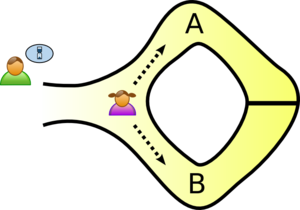
\includegraphics[width=\textwidth]{images/zkp1.png}
        \end{subfigure}
        \hspace{0.25cm}
        \begin{subfigure}{0.25\textwidth}
            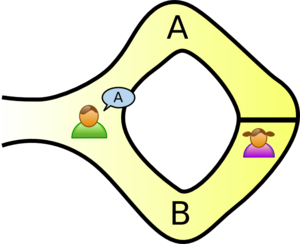
\includegraphics[width=\textwidth]{images/zkp2.png}
        \end{subfigure}
        \hspace{0.25cm}
        \begin{subfigure}{0.25\textwidth}
            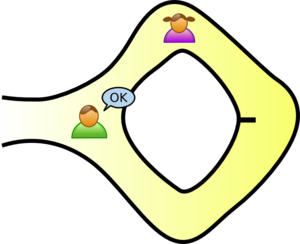
\includegraphics[width=\textwidth]{images/zkp3.png}
        \end{subfigure}
        \caption[Jama Ali Babe.]{Igra Ane in Bojana v jami Ali Babe. Vir slike Wikipedia~\cite{zkp}.}
        \label{fig:alibaba}
    \end{figure}
\end{primer}

Dokazi brez razkritja znanja so torej orodje, s katerim lahko pokažemo, da nekaj vemo, brez da bi 
izdali skrivnost. V osnovi so to interaktivni protokoli med \textit{dokazovalcem} in \textit{preverjevalcem}. 
Dokazovalec želi preverjevalca prepričati, da pozna skrivnost, brez da bi mu jo izdal. Taki protokoli 
sodijo med \textbf{interaktivne dokaze}, kar pomeni, da zadoščajo dvema lastnostima:
\begin{itemize}
    \item \textbf{Kompletnost} (angl.\ \textit{completeness}): Če trditev, ki se dokazuje,
        drži, potem bo preverjevalec sprejel dokaz dokazovalca (če noben od njiju ne bo goljufal).
    \item \textbf{Zadostnost} (angl.\ \textit{soundness}): Če trditev, ki se dokazuje, ne
        drži, potem noben dokazovalec (tudi tak, ki goljufa) ne more predložiti dokaza, ki bi 
        ga preverjevalec sprejel, razen z zelo majhno verjetnostjo.
\end{itemize}
Poleg teh dveh lastnosti, mora dokaz brez razkritja znanja zadoščati še eni, o njej govori že samo ime:
\begin{itemize}
    \item \textbf{Brez razkritja znanja} (angl.\ \textit{zero-knowledge}): Če trditev, ki se dokazuje, 
        drži, potem noben preverjevalec (tudi tak, ki goljufa) ne bo iz dokaza izvedel ničesar več, 
        kot samo to, da trditev drži.
\end{itemize}

\begin{opomba}
    Dokazi brez razkritja znanja niso zares dokazi v matematičnem smislu. Vedno obstaja določena verjetnost, 
    da lahko goljufiv dokazovalec prepriča iskrenega preverjevalca o trditvi, ki ne drži.
\end{opomba}

\todo[
kaj je fiat shamir~\cite{fiat1987heuristic}:  
Če dokazovalec $A$ želi prepričati preverjevalca $B$ o svoji identiteti, lahko uporabi eno od treh
vrst shem:
\begin{itemize}
    \item \textbf{avtentikacijska shema} (angl.\ \textit{authentication scheme}) dovoli $A$, da dokaže
        $B$ svojo identiteto, vendar nihče drug ne more $B$ dokazati, da je $A$.
    \item \textbf{identifikacijska shema} (angl.\ \textit{identification scheme}) dovoli $A$, da dokaže
        $B$ svojo identiteto, vendar more $B$ dokazati nikomur drugemu, da je $A$.
    \item \textbf{podpisna shema} (angl.\ \textit{signature scheme}) dovoli $A$, da dokaže
        $B$ svojo identiteto, vendar niti $B$ ne more sebi dokazati, da je $A$.
\end{itemize}
dokaz varnosti~\cite{pointcheval1996forking}:]
{natančneje o zkp: sigma protocols, \\ zero knowledge proof (of knowledge) fiat-shamir}

Torej, da preprečimo napad na generiranje ključev, od vsakega podpisnika $P_i$ zahtevamo, da poleg 
svojega javnega ključa $I_i$ objavi tudi dokaz o znanju brez razkritja znanja za svoj zasebni ključ 
glede na javni ključ. Objaviti mora torej dokaz, da pozna diskretni logaritem $I_i$ modulo $g$. 
Ta dokaz je neinteraktiven, saj obravnavmo model slučajnega oraklja in lahko uporabimo Fiat-Shamirjevo 
hevristiko.

Ker tovrstni dokazi brez preverjevalca nimajo smisla, se na tej točki vredno vprašati, kdo bo preverjal 
veljavnost dokazov. Izkaže se, da je najbolj enostavno, da se dokaze doda v posamezne javne ključe. 
Tako pade breme preverjanja na tistega, ki bo preverjal podpis. Problematično je dejstvo, da taka 
sprememba podaljša javne ključe in privede do izgube učinkovitosti. Preverjanje veljavnosti podpisa 
bo sedaj poleg dveh modularnih potenciranj potrebovalo še dodatnih $2|S|$, saj je potrebno preveriti 
vse dokaze javnih ključev. Posamezni preverjevalec podpisov lahko sicer dodatno delo opravi le enkrat 
za vsako skupino, če natančno beleži rezultate preverjanja dokazov.

\subsubsection{Učinkovitost podpisovanja: Merklova drevesa}
Za dokaz varnosti je potrebno, da lahko algoritem, ki bo simuliral proces podpisovanja in napadanja 
(pogosto se tak algoritem imenuje \textit{simulator}), v polinomskem času za vsakega pokvarjenega 
podpisnika $P_j$ pridobi diskretni logaritem $I_j$ iz predloženega dokaza o znanju brez razkritja 
znanja. Izkaže pa se, da če je $P_j$ dokaz izračuna s $q$ klici slučajnega oraklja, potem simulator 
uspešno pridobi diskretni logaritem z verjetnostjo največ $1/q$. Torej, če je $k$ pokvarjenih 
podpisnikov, bo simulator uspešen z verjetnostjo največ $1/q^k$. Z drugimi besedami, če želimo 
polinomski simulator, je podpisnikov lahko največ logaritemsko mnogo v številu klicev oraklja $q$.

\todo{kaj pomeni logaritemsko mnogo - je to prav?}

Ta problem lahko rešimo tako, da vsak podpisnik $P_i$ najprej izračuna svoj par ključev $(s_i, I_i)$ 
in tudi zavezo $X_i$. Potem si vsi izmenjajo $I_i$ in $X_i$. Vsak podpisnik lahko sedaj izračuna 
\textit{skupni izziv} 
$$ 
e = H(X_1 || I_1 || X_2 || I_2 || \dots || X_L || I_L).
$$
Podpisniki za dokaz znanja sedaj uporabijo Schnorrov podpis $e$ s svojim parom ključev. 
\todo{a to pravilno razumem?}
To pomeni, da za generiranje dokazov $k$ pokvarjenih podpisnikov sedaj rabi le $kq$ klicev oraklja, 
torej je polinomski simulator uspešen z verjetnostjo $1/kq$. To omogoča, da je podpisnikov več 
kot logaritemsko mnogo. Pojavi pa se drugačen problem z učinkovitostjo, saj mora sedaj vsak podpisnik 
v svojem javnem ključu hraniti še Schnorrov podpis sporočila $e$ in pa tudi vse javne ključe 
sopodpisnikov in njihove zaveze. Brez teh podatkov namreč dokaz znanja (Schnorrov podpis) ni preverljiv. 
To pomeni, da je za katerokoli podskupino $S$ velikost ključa proporcionalna velikosti celotne skupine 
$G$. Poleg tega mora sedaj preverjevalec preveriti, da se vsi vektorji javnih ključev ujemajo. V primerjavi 
z osnovno naivno idejo, kjer je preverjevalec potreboval le $|S|$ navadnih Schnorrovih javnih ključev, 
je v tej izvedbi velikost javnega ključa nedopustno velika.

Da nazaj pridobimo učinkovit podpis, se lahko zanesemo na slučajnega oraklja in kriptografsko 
orodje, imenovano \textbf{Merklovo drevo} (angl.\ \textit{Merkle tree}). V osnovi je to 
\textit{binarno drevo}, torej drevo, kjer ima vsako vozlišče največ dva otroka. Ideja je, da v liste 
shranimo zgostitve katerekolih podatkov, pridobljene s pomočjo izbranega slučajnega oraklja ali zgoščevalne 
funkcije. Drevo potem gradimo navzgor tako, da v vsako vozlišče shranimo zgostitev stika zgostitev levega in desnega 
otroka. Tako nadaljujemo do korena. Pomembno je, da je za pridobivanje zgostitev uporabljena zgoščevalna 
funkcija, ki je skoraj brez trčenj ali pa slučajni orakelj. Osnovna 
struktura je prikazana na sliki~\ref{fig:merkle}.
\begin{figure}[ht]
  \centering
  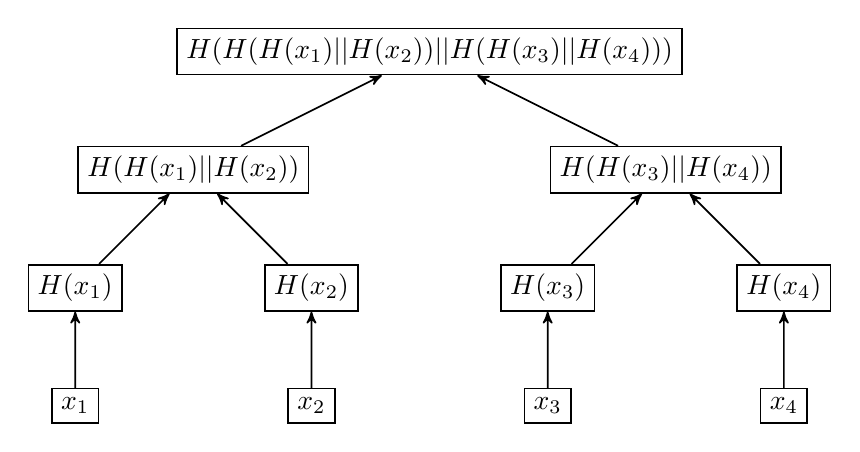
\begin{tikzpicture}[<-, >=stealth', auto, semithick,
   level/.style={sibling distance=60mm/#1}]

  \node [rectangle,draw] {$H(H(H(x_1) || H(x_2)) || H(H(x_3) || H(x_4)))$}
    child {node [rectangle,draw] {$H(H(x_1) || H(x_2))$}
        child {node [rectangle,draw] {$H(x_1)$}
            child {node [rectangle,draw] {$x_1$}}
        }
        child {node [rectangle,draw] {$H(x_2)$}
            child {node [rectangle,draw] {$x_2$}}
        } 
    }
    child {node [rectangle,draw] {$H(H(x_3) || H(x_4))$}
        child {node [rectangle,draw] {$H(x_3)$}
            child {node [rectangle,draw] {$x_3$}}
        } 
        child {node [rectangle,draw] {$H(x_4)$}
            child {node [rectangle,draw] {$x_4$}}
        }
    };
  \end{tikzpicture}
  \caption[Merklovo drevo.]{Primer Merklovega drevesa s štirimi listi. Imamo torej $4$ vhodne podatke
    $x_1, x_2, \dots, x_4$, na vsakem nivoju drevesa se izračuna stik in zgostitev. Ustvarjeno s 
    pomočjo~\cite{SOtikz}.}
  \label{fig:merkle}
\end{figure}

Pomembno je opaziti, da če zgoščevalna funkcija ustvarja zgostitve, dolge $k$ bitov, bodo toliko 
dolgi vsi podatki, ki jih hranijo vsa vozlišča drevesa. Za Merklova drevesa je ključno, da je v primeru 
varne zgoščevalne funkcije računsko zelo težko spremeniti katerokoli vrednost v drevesu, brez da bi se 
spremenila vrednost v korenu. Enako velja za spremembe vhodnih podatkov. Merklova drevesa nam torej 
omogočajo, da se zavežemo $L$ vrednostim $x_1, x_2, \dots, x_L$ tako, da enostavno vrnemo en sam 
$k$-bitni niz. To storimo tako, da shranimo zgostitve vrednosti $x_1, x_2, \dots, x_L$ v liste drevesa 
in izračunamo koren. Vrednostim se zavežemo tako, da preverjevalcu damo vrednost korena. Ko mu kasneje 
želimo razkriti vrednosti, mu jih enostavno povemo, on pa lahko z izračunom drevesa preveri, da so 
vrednosti prave. Povzeto po~\cite{micali2000csproofs}.

\begin{trditev}[Overjevalna pot~\cite{micali2000csproofs}]
\label{trd:overjevalna_pot}
    Naj bo $A$ zavezovalec, ki se želi zavezati vrednostim $x_1, x_2, \dots, x_L$ preverjevalcu $B$. Če 
    se $A$ zaveže tako, da $B$ pove vrednost korena Merklovega drevesa, izračunanega na podlagi 
    vrednosti $x_1, x_2, \dots, x_L$, potem lahko dokaže zavezo eni vrednosti $x_i$ ($1 \le i \le L$)
    tako, da preverjevalcu $B$ pove $1 + \lceil \log L \rceil$ vrednosti: $x_i$ in pa \textbf{overjevalno 
    pot}, torej vrednosti, shranjene v sestrskih vozliščih vseh vozlišč na poti med vključno $x_i$ in 
    korenom (brez korena, ki ga $B$ že pozna).
\end{trditev}

\begin{dokaz}
    Trditev lahko dokažemo z indukcijo na globino Merklovega drevesa $d$. Naj bo $x$ vrednost, za katero
    želimo dokazati zavezo in $w_1, w_2, \dots, w_d$ overjevalna pot.
    \begin{itemize}
        \item $d = 2$: Če je globina drevesa $2$, želimo pokazati, da moramo poleg $x$ povemo samo eno  
            dodatno vrednost. Ta vrednost je torej zgostitev $x$-ove sosednje vrednosti $y$. Ko $B$ izračuna
            $H(x || y)$, je to že koren, in lahko vrednost primerja z zabeleženo.
        \item $n \rightarrow n + 1$: Predpostavimo torej, da za globino drevesa $n$ lahko preverimo zavezo s 
            podanimi $1 + d$ vrednostmi. To nam omogoča izračuna vrednosti v enem od korenovih otrok v 
            drevesu globine $n + 1$, po indukcijski predpostavki. Če poznamo še vrednost drugega otroka, je 
            možen izračun korena.
    \end{itemize}
\end{dokaz}

Merklova drevesa lahko sedaj uporabimo, da naredimo večstranski podpis bolj učinkovit. Podpisniki
še vedno predložijo dokaze znanja prek Schnorrovega podpisa, po izmenjavi dokazov pa vsak izračuna 
Merklovo drevo z listi $I_1, I_2, \dots, I_L$. To drevo bo torej globine $\log L$. Za svoj javni 
ključ potem vsak podpisnik $P_i$ nastavi $I_i$ in overjevalno pot za $I_i$. Ker je ponavadi $I_i$ 
veliko daljši od dolžine zgostitev, in ker je v overjevalni poti le $\log L$ zgostitev, se ključ 
ne podaljša veliko (npr.\, če je $I_i$ dolg $2000$ bitov in so zgostitve $200$-bitne, bo $1000$ 
podpisnikov ustvarilo ključe, dolge manj od $4000$ bitov, torej manj kot dvakrat daljše).

Ko sedaj preverjevalec preverja podpis sporočila $m$ s strani $S$, lahko za vsakega podpisnika 
izračuna vrednost korena Merklovega drevesa in preveri, da se vse ujemajo. Obstoj enega nepokvarjenega
podpisnika tako prisili vse pokvarjene, da uporabljajo prave ključe (ali pa najdejo trk v 
zgoščevalni funkciji, kar je izjemno težko). S to spremembo smo tako uspešno ohranili podpise 
varne in časovno učinkovite.

\subsection{Definicija večstranskega Schnorrovega podpisa}
\label{sec:def_multi_schnorr}
Sedaj smo pripravili vse potrebno, da podamo natančno definicijo končne sheme. 

\subsubsection{Skupni parametri}
Vsi podpisniki se strinjajo o skupnem varnostnem parametru $k$ in sekundarnem varnostnem parametru
$k'$, ki je deterministično izračunan iz $k$ (ponavadi kar $k' = 100$). Za velikost $L$ skupine podpisnikov
$G$ predpostavimo, da je polinomska v $k$.

Shemo obravnavamo v modelu slučajnega oraklja, tako da imajo vsi podpisniki dostop do slučajnega
oraklja $H$. Na dogovorjen način ga uporabijo, da ustvarijo pet neodvisnih orakljev
\begin{align*}
    H_1, H_2: \{0, 1\}^* &\rightarrow \{0, 1\}, \\
    H_3, H_5: \{0, 1\}^* &\rightarrow \{0, 1\}^{k'}, \\
    H_4: \{0, 1\}^* &\rightarrow \{0, 1\}^{2k'}.
\end{align*}
Prav tako predpostavimo, da imajo vsi podpisniki dostop do algoritma $GenPrimes(k)$~\ref{alg:gen}.

Za lažjo obravnavo si izberemo še enega izmed podpisnikov, in ga označimo z $D$. Ta podpisnik bo 
vrnil končni podpis, ne ve pa nobenih dodatnih skrivnosti. $D$ lahko tudi predstavlja vse podpisnike, 
a je opis sheme malce lažji, če si izberemo enega -- v tem primeru je on prejemnik vseh sporočil
ostalih podpisnikov, svoje odgovore pa potem oddaja (angl.\ \textit{broadcast}) ostalim podpisnikom.
Če si ne izberemo podpisnika $D$, si podpisniki sporočila pošiljajo v krogu (vsak pošlje svoje sporočilo
desnemu sosedu, ko prejme sporočilo levega, spet pošlje desnemu. Vsak torej pošlje $L$ sporočil, na
koncu imajo vsi vse potrebne podatke za izračune).

\subsubsection{Generiranje ključev}
Vsi podpisniki morajo sami generirati parametre $p, q$ in $g$. Za prva dva uporabijo algoritem 
$GenPrimes(k)$~\ref{alg:gen}. Za izvor naključnosti uporabijo zaporedje $H_1(2^k), H_1(2^k + 1), \dots$.
Za generiranje elementa $g$ reda $q$ uporabijo izvor naključnosti $H_2(2^k), H_2(2^k + 1), \dots$.

Ko ima vsak podpisnik $P_i$ ($1 \le i \le L$) na voljo skupne parametre, si izbere svoj zasebni 
ključ $s_i \in [0, q - 1]$ in izračuna
$$ 
I_i = g^{s_i} \bmod p.
$$
Do tu je postopek enak, kot pri naivni verziji. Da preprečimo napad na generiranje ključev, mora 
vsak podpisnik na tem mestu izbrati naključen $r_i \in [0, q- 1]$ in izračunati zavezo
$$ 
X_i = g^{r_i} \bmod p.
$$
Potem si podpisniki med seboj izmenjajo vrednosti $(X_i, I_i)$. Vsak na tem mestu lahko izračuna
\begin{align*}
    e &= H_3(X_1 || I_1 || X_2 || I_2 || \dots || X_L || I_L), \\
    y_i &= e s_i + r_i,
\end{align*}
in pošlje $y_i$ vsem ostalim podpisnikom. Vsak podpisnik je na tem mestu prejel Schnorrove podpise
(in s tem dokaze znanja brez razkritja znanja) zasebnih ključev vse ostalih podpisnikov. Na tem mestu
mora torej $P_i$ preveriti veljavnost vseh podpisov $(X_j, y_j)$ vseh ostalih podpisnikov $P_j$ 
($1 \le j \le L$). To stori s standardnim izračunom za preverjanje Schnorrovega podpisa~\eqref{eq:schnorr-ver}: 
$$
g^{y_j} \stackrel{?}{\equiv} X_j \cdot I_j^{e} \pmod p.
$$

Ko podpisnik $P_i$ ugotovi, da so vsi podpisi veljavni, lahko izračuna Merklovo drevo, ki ima v 
listih po vrsti razporejene $I_1, I_2, \dots, I_L$ in za svojo zgoščevalno funkcijo uporablja $H_4$.
Ko je drevo izračunano, $P_i$ prebere overjevalno pot $\text{pot}_i$ svojega ključa $I_i$ in vrne 
javni ključ
$$ 
\text{pk}_i = (p, q, g, I_i, \text{pot}_i).
$$

\subsubsection{Podpisovanje}
Naj bo $S = \{P_{id_1}, P_{id_2}, \dots, P_{id_l}\}$ podksupina velikosti $l$ skupine $G$, ki želi 
večstransko podpisati sporočilo $m$. To lahko storijo s tremi krogi komunikacije:
\begin{enumerate}
    \item Vsak podpisnik $P_{id_j} (1 \le j \le l)$ si izbere naključno število $r_j \in [0, q - 1]$ 
        in izračuna zavezo
        $$ 
        X_j = g^{r_j} \bmod p.
        $$
        Zavezo $X_j$ nato pošlje podpisniku $D$.
    \item $D$ izračuna skupno zavezo
        $$ 
        \tilde{X} = (X_1 \cdot X_2 \cdot \cdots \cdot X_l) \bmod p
        $$
        in jo pošlje vsem podpisnikom $P_{id_j} (1 \le j \le l)$.
    \item Vsak podpisnik $P_{id_j} (1 \le j \le l)$ izračuna
        \begin{align*}
            e &= H_5(\tilde{X} || m || S), \\
            y_j &= e s_j + r_j
        \end{align*}
        in pošlje $y_j$ podpisniku $D$.
\end{enumerate}
Na tem mestu ima $D$ vse kar rabi, da dokonča podpis. Najprej izračuna
$$
\tilde{y} = (y_1 + y_2 + \cdots + y_l) \bmod q
$$
in nato vrne končni podpis
$$
\sigma = (\tilde{X}, \tilde{y}).
$$

\subsubsection{Preverjanje}
Preverjanje je podobno naivni verziji, le da je potrebno dodatno preveriti ustreznost Merklovih
korenov. Če torej preverjevalec želi preveriti veljavnost podpisa $\sigma = (\tilde{X}, \tilde{y})$
sporočila $m$, moramo predpostaviti, da lahko dostopa do vseh javnih ključev $\{\text{pk}_{id_1},
\text{pk}_{id_2}, \dots, \text{pk}_{id_l}\}$ vseh podpisnikov $S = \{P_{id_1}, P_{id_2}, \dots, 
P_{id_l}\}$.

Najprej mora preverjevalec preveriti, da se vseh $l$ izvodov skupnih parametrov $p, q$ in $g$ ujema.
Da dokončno potrdi veljavnost in ustreznost javnih ključev, za vsakega podpisnika $P_{id_j} (1 \le
j \le l)$ s pomočjo $I_{id_j}$ in $\text{pot}_{id_j}$ izračuna vrednost $V_{id_j}$ v korenu 
Merklovega drevesa, kot prikazano v trditvi~\ref{trd:overjevalna_pot}. Ko izračuna vse vrednosti
$V_{id_j}$, mora preveriti, da so vse enake. 

Ko se preverjevalec prepriča o veljavnosti ključev, postopa podobno kot pri naivni verziji. Najprej
mora izračunati
$$
\tilde{I}_S = (I_{id_1} \cdot I_{id_2} \cdot \cdots \cdot I_{id_l}) \bmod p.
$$
Če si dosledno beleži izračune, lahko preverjevalec ta del preverjanja podpisa opravi le enkrat za
vsako skupino podpisnikov $S$.

Potem mora preverjevalec izračunati izziv s pomočjo slučajnega oraklja
$$
e = H_5(\tilde{X} || m || S)
$$
in preveriti, če velja
\begin{equation}
\label{eq:asm-check}
g^{\tilde{y}} \stackrel{?}{\equiv} \tilde{X} \tilde{I}_S^e \pmod p.
\end{equation}

Če je torej podpis $\sigma = (\tilde{X}, \tilde{y})$ veljaven podpis sporočila $m$, lahko levo stran
enačbe~\eqref{eq:asm-check} zapišemo kot
\begin{align*}
    g^{\tilde{y}} \bmod p &= g^{(y_1 + y_2 + \cdots + y_l) \bmod q} \bmod p \\
                          &\stackrel{\ref{trd:mod-q}}{=} g^{y_1 + y_2 + \cdots + y_l} \bmod p \\
                          &= g^{e s_1 + r_1 + e s_2 + r_2 + \cdots + e s_l + r_l} \bmod p \\
                          &= g^{r_1 + r_2 + \cdots r_l} g^{e (s_1 + s_2 + \cdots s_l)} \bmod p,
\end{align*}
desno pa po trditvi~\ref{trd:mod-mn-pt}
\begin{align*}
    \tilde{X} \tilde{I}_S^e \bmod p &= ((X_1 \cdot X_2 \cdot \cdots \cdot X_l) \bmod p)
        ((I_{id_1} \cdot I_{id_2} \cdot \cdots \cdot I_{id_l}) \bmod p)^e \bmod p \\
    &=((g^{r_1} \bmod p \cdot g^{r_2} \bmod p \cdot \cdots \cdot g^{r_l} \bmod p) \bmod p) \cdot \\
    &\cdot ((g^{s_1} \bmod p \cdot g^{s_2} \bmod p \cdot \cdots \cdot g^{s_l} \bmod p) \bmod p)^e \bmod p \\
    &\stackrel{\ref{trd:mod-mn-pt}}{=} (g^{r_1} \cdot g^{r_2} \cdot \cdots \cdot g^{r_l}) \bmod p) 
        ((g^{s_1} \cdot g^{s_2} \cdot \cdots \cdot g^{s_l}) \bmod p)^e \bmod p \\
    &\stackrel{\ref{trd:mod-mn-pt}}{=} (g^{r_1} \cdot g^{r_2} \cdot \cdots \cdot g^{r_l}) 
        (g^{s_1} \cdot g^{s_2} \cdot \cdots \cdot g^{s_l})^e \bmod p \\
    &= g^{r_1 + r_2 + \cdots r_l} g^{e (s_1 + s_2 + \cdots s_l)} \bmod p.
\end{align*}
Ker se leva in desna stran ujemata, enačba~\eqref{eq:asm-check} pravilno preveri pravilnost večstranskega
Schnorrovega podpisa.

\subsection{Varnost večstranskega Schnorrovega podpisa}
\label{sec:proof_multi_schnorr}
Dokazati si želimo, da je shema, definirana v zgornjem razdelku~\ref{sec:def_multi_schnorr} \textit{varna},
torej ustreza pogojem definicije varnosti~\ref{def:asm-varnost}, kjer ima napadalec $F$ sposobnosti,
definirane v~\ref{def:asm-napadalec}. Varnost torej pomeni, da je preprečeno eksistencialno ponarejanje,
zaradi napadalčevega nadzora nad komunikacijskim omrežjem pa si lahko privošči napad z izbranimi sporočili.
Še več, ker se ukvarjamo z večstranskimi podpisi, si napadalec lahko izbere še podskupino, ki bo 
sporočilo podpisovala. Napadalec lahko torej na katerikoli točki od katerekoli podskpupine zahteva
podpis kateregakoli izbranega sporočila.

Zaradi kompleksnosti napadalca, dokaz varnosti poteka tako, da najprej dokažemo ekvivalentnost med
šibkejšim napadalcem $F'$ in prvotnim napadalcem $F$, potem pa dokažemo varnost v primeru šibkega
napadalca $F'$.

\subsubsection{Šibek napadalec}
Za enostavnejšo analizo definiramo \textbf{šibkega napadalca} (ali nasprotnika) (angl.\ 
\textit{weak adversary}) $F'$. Njegov cilj je enak izvornemu napadalcu $F$. Želi si torej ponarediti podpis
s pomočjo napada z izbranim sporočilom in podskupino. Izbere si lahko podpisnika, in od njega
zahteva podpis izbranega sporočila skupaj z izbrano podskupino $S$. Napadalca se razlikujeta v tem,
da je $F'$ bistveno šibkejši, oz.\ ima manj nadzora nad potekom podpisovanja in komunikacijo med
podpisniki.

Šibek napadalec nima zmožnosti pokvariti podpisnikov. Vse, kar lahko stori $F'$ je, da si preden skupina
generira svoje ključe, izbere podpisnika $P_i$, ki ga bo napadal. Edina interakcija, ki je potem dovoljena
šibkemu napadalcu, je s podpisnikom $P_i$. Ko je podpisnik napaden, mora zanj $F'$ priskrbeti vse vhode
za algoritme in vse vhodna sporočila, ki jih prejme. Prav tako lahko vidi vsa poslana sporočila
podpisnika. Situacija je torej taka, kot da ostali podpisniki sploh ne obstajajo, pri podpisovanju 
sodleujeta samo $P_i$ in $F'$. Ko podpisnik $P_i$ generira svoj ključ, $F'$ nad njim izvede napad z izbranim 
sporočilom in podskupino.

Ker mora šibek napadalec za izbranega podpisnika predložiti vse vhode in komunikacijo, lahko vidimo
delovanje šibkega napadalca kot delovanje napadalca, ki pokvari vse podpisnike, razen podpisnika $P_i$.
V obeh primerih bo podpisnik $P_i$ v podpisu sodeloval le z napadalcem, ki zanj nadzoruje celoten
potek podpisovanja. Ta povezava tipov napadalcev je formalno opisana v izreku~\ref{izr:šibka-varnost}.
Pred dokazom izreka pa moramo, tako kot za napadalca $F$, tudi tu definirati kaj pomeni varnost sheme.

\begin{definicija}[Šibka varnost]
    Naj bo $k$ varnostni parameter (ki si ga delijo vsi podpisniki). Naj bo $c > 0$ poljubna konstanta. 
    Naj bo $F'$ šibek napadalec, ki je omejen s polinomskim časom v parametru $k$. Naj bo $p$ 
    verjetnost, da $F'$ vrne trojico $(\sigma, m, S)$, za katero velja: 
    \begin{itemize}
        \item $\sigma$ je veljaven večstranski podpis sporočila $m$ s strani skupine $S$.
        \item Obstaja nepokvarjen podpisnik $P$ iz skupine $S$, od katerega $F'$ ni zahteval podpisa 
            sporočila $m$ s strani skupine $S$.
    \end{itemize}
    Shemi za večstranske 
    podpise podskupine z odgovornostjo bomo rekli, da je \textbf{šibko varna}, če velja 
    $$ 
    p < k^{-c}.
    $$
\end{definicija}

Sedej imamo vse potrebno, da dokažemo ekvivalentnost šibke varnosti in varnosti, in s tem
ekvivalentnost šibkega napadalca in napadalca.

\begin{izrek}
\label{izr:šibka-varnost}
    Naj bo $Q$ tak polinom, da je pri poljubno izbranem varnostnem parametru $k$ za velikost $L$ 
    skupine podpisnikov $G$ velja
    $$
    L < Q(k).
    $$
    Potem je večstranski Schnorrov podpis iz razdelka~\ref{sec:def_multi_schnorr} varen natanko
    tedaj, ko je šibko varen.
\end{izrek}

\begin{dokaz}
    Ker se definicija varnosti in šibke varnosti razlikuje le v uporabi napadalca $F$ ali šibkega
    napadalca $F'$, je potrebno pokazati le, da sta $F$ in $F'$ ekvivalentna (ob ustrezni velikost
    skupine podpisnikov).

    $(\Rightarrow)$: Predpostavimo, da podpis ni šibko varen. Kot smo že prej smo omenili, je delovanje
    šibkega napadalca $F'$ enako delovanju napadalca $F$, ki pokvari vse podpisnike razen enega.
    Napadalec $F$ ima torej vse zmožnosti, ki jih ima napadalec $F'$ (in še mnogo več). Če podpis ni
    šibko varen, lahko $F$ s simulacijo $F'$, opisano zgoraj, z nezanmarljivo verjetnostjo vrne
    ponarejen podpis, torej sheam tudi ni varna.

    $(\Leftarrow)$: Predpostavimo, da podpis ni varen. Obstaja torej napadalec $F$, ki je omejen
    s polinomskim čason v parametru $k$ in uspešno izvede napad z izbranim sporočilom in podskupino.
    Na tej točki omenimo še, da je za smiselen ponaredek podpisa potrebno, da pri podpisovanju sodeluje
    vsaj en nepokvarjen podpisnik. Sicer je napadalec edini ki podpisuje, zato varnost sheme ni ogrožena.
    Če pa pri podpisovanju sodeluje iskren podpisnik, in napadalec uspešno ustvari ponaredek, pa
    to kaže na težave v varnosti.

    Konstruirajmo šibkega napadalca $F'$, ki deluje tako, da pred začetkom podpisovanja izbere naključnega
    podpisnika $P_i$ ($1 \le i \le L$) za tarčo svojega napada. $F'$ se torej za podpisnika $P_i$ postavi
    v vlogo vseh ostalih podpisnikov. $F'$ lahko torej $F$ simulira delovanje vseh podpisnikov razen
    $P_i$. Če se $F$ odloči pokvariti kateregakoli podpisnika, ki ni $P_i$, mu lahko $F'$ posreduje
    potrebne zasebne informacije. Podobno tudi, če si $F$ izbere podpisnika (razen $P_i$) za tarčo napada z
    izbarnim sporočilom in podskupino. V primeru, da je tarča napada $P_i$, $F'$ prejme zahtevek za
    napad od $F$ in ga posreduje podpisniku $P_i$, ta pa normalno pošlje svoj odgovor napadalcu $F$.

    Ko $F$ konča svoj napad, vrne trojico $(\sigma, m, S)$. Če je to veljaven ponaredek, jo vrne tudi
    šibek napadalec $F'$. Če ponaredek ni veljaven, če $P_i$ ni eden izmed podpisnikov v $S$, ali pa
    če je $P_i$ tekom podpisovanja pokvarjen s strani $F$, je šibek napadalec neuspešen pri svojem napadu.
    Poglejmo si verjetnost, da $F'$ uspe pri svojem napadu:
    \begin{align*}
          &\text{Pr}(\text{$F'$ vrne veljaven ponaredek}) = \\
        = &\text{Pr}(\text{$F$ vrne veljaven ponaredek } \cap \text{ $P_i \in S$ in ni pokvarjen}) \\
        = &\sum_{i=1}^L \text{Pr}(\text{$F'$ izbere $P_i$}) \cdot 
            \text{Pr}(\text{$F$ vrne veljaven ponaredek } \cap \text{ $P_i \in S$ in ni pokvarjen}) \\
        = &\sum_{i=1}^L \frac{1}{L} \cdot 
            \text{Pr}(\text{$P_i \in S$ in ni pokvarjen | $F$ vrne veljaven ponaredek}) \\
          &\cdot \text{Pr}(\text{$F$ vrne veljaven ponaredek}) \\
        \geq &\frac{1}{L} \cdot \text{Pr}(\text{$F$ vrne veljaven ponaredek}),
    \end{align*}
    kjer smo pri prehodu iz tretje v četrto vrstico uporabili osnovno lastnost verjetnosti, ki pravi
    $$
    \text{Pr}(A \cap B) = \text{Pr}(A \text{ }|\text{ } B) \cdot \text{Pr}(B),
    $$
    pri prehodu v zadnjo vrstico pa smo upoštevali, da velja
    \begin{equation}
    \label{eq:geq1}
    \sum_{i=1}^L \text{Pr}(\text{$P_i \in S$ in ni pokvarjen | $F$ vrne veljaven ponaredek}) \geq 1.
    \end{equation}
    Neenačba~\eqref{eq:geq1} drži, saj mora pri uspešnem ponarejanju sodelovati vsaj en nepokvajren
    podpisnik. Če torej $F$ vrne veljaven ponaredek, bo vsaj ena od verjetnosti v zgornji vsoti enaka $1$.

    Pri ponarejanju je torej $F$ uspešen največ $L$-krat več kot $F'$, kar pomeni, da shema ni šibko
    varna.
\end{dokaz}

\subsubsection{Dokaz varnosti}
Ker sta napadalec in šibek napadalec ekvivalentna, je dovolj pokazati varnost v primeru šibkega
napadalca, shema pa je potem tudi varna po izreku~\ref{izr:šibka-varnost}.

\begin{izrek}[Varnost večstranskega Schnorrovega podpisa]
    Če drži predpostavka o težavnosti diskretnega logaritma pri ASM~\ref{def:asm_dlp}, je večstranski 
    Schnorrov podpis, definiran v razdelku~\ref{sec:def_multi_schnorr}, varen.
\end{izrek}

Želimo torej pokazati, da če obstaja šibek napadalec, ki je omejen s polinomskim časom v parametru
$k$, potem obstaja nek algoritem $A$, ki prav tako teče v polinomskem času, s katerim lahko prekršimo
predpostavko o diskretnem logaritmu pri ASM. Bolj specifično, prekršimo lahko predpostavko o
težavnosti PDL. $A$ je torej algoritem, ki za vhod prejme $p, q, g$ in $I$, in vrne $s \in [0, q - 1]$,
da velja $g^s \equiv I \pmod q$. Ideja je, da $A$ simulira podpisovanje za šibkega napadalca,
ki vrne ponarejen podpis, iz katerega $A$ lahko razbere diskretni logaritem, ki ga išče.

Bolj specifično, med svojim delovanjem šibki napadalec opravlja dve vrsti poizvedb. Prva je
\textit{zgoščevalna poizvedba}, kjer napadalec pošlje slučajnemu oraklju nek niz, ta pa mu odgovori
z njegovo zgostitvijo. $A$ lahko simulira odgovor na tovrstne poizvedbe z vračanjem naključnih odgovorov.

Druga vrsta poizvedb je \textit{podpisovalna poizvedba}, kjer napadalec podpisniku $P_i$ (ki ga je 
izbral na začetku) pošlje sporočilo $m$ in skupino $S$, ta pa mu nazaj pošlje zavezo $X_i$. Potem
mora napadalec igrati vlogo podpisnika $D$, ki agregira informacije. Podpisniku $P_i$ pošlje skupno
zavezo $\tilde{X}$, nazaj pa dobi $y_i$. Podpisovalne poizvedbe torej potekajo v dveh krogih in
predstavljajo izvedbo napada z izbranim sporočilom in podskupino nad podpisnikom $P_i$.

Za lažjo konstrukcijo algoritma $A$, je smotrno šibkega napadalca $F'$ še dodatno poenostaviti. Naj
$q_{\text{zgoščevalna}}$ označuje največje število zgoščevalnih poizvedb, ki jih opravi $F'$,
$q_{\text{podpisovalna}}$ pa največje število podpisovalnih. Poenostavljen napadalec $\mathcal{F}$
deluje popolnoma enako kot $F'$, le da pred drugim krogom podpisovalne poizvedbe $\mathcal{F}$
najprej pošlje zgoščevalno poizvedbo slučajnemu oraklju $H_5$ z vhodom $(\tilde{X}, m, S)$. Podobno,
preden $\mathcal{F}$ vrne ponarejen podpis $(\tilde{X}, \tilde{y})$ sporočila $m_F$, najprej opravi
zgoščevalno poizedbo pri slučajnemu oraklju $H_5$ z vhodom $(\tilde{X}, m_F, S)$. Tako $\mathcal{F}$
vsaki podpisovalni poizvedbi in ponaredku dodeli zgostitev. Ker opravi $q_{\text{podpisovalna}}$
podpisovalnih poizvedb in $q_{\text{zgoščevalna}} + q_{\text{podpisovalna}} + 1$ zgoščevalnih in
ker $F'$ po predpostavki teče v polinomskem času, tudi $\mathcal{F}$ teče v polinomskem času.
Dodatno predpostavimo še, da $\mathcal{F}$ po vsaki zgoščevalni poizvedbi shrani odgovor, zato vsako
zgoščevalno poizvedbo za določen vhod opravi le enkrat. Število klicev oraklja $H_5$ označimo s $q_H$.
$A$ bo za delovanje uporabljal napadalce $\mathcal{F}$, saj bo tako za vsak potencialni ponaredek in
vsak napad prejel predogled rezultata prek zgostitve, ki jo vrne $H_5$.

$A$ mora torej znati odgovoriti na vse poizvedbe poenostavljenega napadalca $\mathcal{F}$. Na zgoščevalne 
poizvedbe odgovarja naključno, s pomočjo vnaprej izbranih simuliranih odgovorov $e_1, e_2, \dots, 
e_{q_H}$ oraklja $H_5$. Odgovor na podpisovalno poizvedbo za podpisnika $P_i$ na vhodu $m$ in $S$
je malce bolj zapleten. $A$ stori sledeče:
\begin{enumerate}
    \item Shrani konfiguracijo poenostavljenega napadalca $\mathcal{F}$.
    \item \label{rewind} Si izbere naključen odgovor $e_j$ ($1 \le j \le q_H$) oraklja $H_5$, 
        v upanju, da bo to zgostitev, ki bo identificirala to poizvedbo.
    \item Si izbere naključen $y \in [0, q - 1]$.
    \item Izračuna 
        $$
        X_i = I_i^{-e_j}g^y \bmod p
        $$
        in pošlje $X_i$ v odgovor prvega kroga poizvedbe poenostavljenemu napadalcu $\mathcal{F}$.
    \item Po prejetju $\tilde{X}$ od $\mathcal{F}$ preveri, če $e_j$ ustreza poizvedbi na vhodu
        $(\tilde{X}, m, S)$. Če ja, vrne $y$, sicer se vrne na korak~\ref{rewind}.
\end{enumerate}
Zgornje je primer splošne metode za analiziranje varnosti v kriptografiji, ki se imenuje 
\textbf{previjanje nazaj} (angl.\ \textit{rewinding}). Popularna je pri analizi dokazov brez razkritja
znanja in pri dokazih varnosti v modelu slučajnega oraklja. Metoda dovoli, da prek naključnih izbir
algoritem odgovori na poizvedbo, preden je postavljena, za ceno največ toliko previjanj, kot ima
poizvedba odgovorov.

V tem primeru je previjanje nazaj nujno potrebno za simuliranje iskrenega podpisnika $P_i$. To je zato,
ker je izbira $\tilde{X}$ s strani $\mathcal{F}$ tista, ki odloči izziv $e$, ki ga $P_i$ uporabi za
izračun $y_i$. Algoritem $A$ pa mora zavezo $X_i$ poslati v prvem krogu poizvedbe, preden je znano,
kaj bo izziv $e$. Zato mora uganiti, kater odgovor oraklja $H_5$ bi bil pravi. Ker je možnih vrednosti
$q_H$, bo v najslabšem primeru potreboval $q_H$ previjanj.

Sedaj lahko konstruiramo algoritem $A$ na podlagi poenostavljenega napadalca $\mathcal{F}$. $A$ torej
prejme instanco problema diskretnega logaritma s podatki $p, q, g$ in $I$ (kot predstavljeno v 
definiciji~\ref{def:asm_dlp}). $P_i$ naj označuje podpisnika, ki ga poenostavljen napadalec napada
(to je torej edini nepokvarjeni podpisnik). Ker ima $A$ absoluten nadzor, lahko brez problema
nastavi oraklja $H_1$ in $H_2$ tako, da so $p, q$ in $g$ točno deljeni parametri pri večstranskem
Schnorrovem podpisu. Potem lahko izbere $I_i = I$ in nastavi $H_3$ tako, da lahko dokaže znanje
diskretnem logaritmu $I_g$ modulo $g$. \todo{to si lahko malo razjasnemo}. Tu naletimo na podoben
problem, kot pri odgovarjanju na druge kroge podpisovalnih poizvedb. $A$ mora poslati zavezo $X_i$
preden pozna skupni izziv $e$. Problem ponovno rešimo s previjanjem poenostavljenega napadalca
$\mathcal{F}$. Previti je treba največ tolikokrat, kot je poizvedb, ki jih $\mathcal{F}$ pošlje
$H_3$ (označimo $q_{H_3}$).

Potem lahko $A$ požene $\mathcal{F}$ in odgovarja na njegove poizvedbe kot opisano zgoraj. Ideja
dokaza od tu naprej je, da ko $\mathcal{F}$ vrne ponarejen podpis, $A$ uporabi previjanje in
\textbf{lemo o razcepu}~\ref{izr:forking} (angl.\ \textit{forking lemma}), da pridobi še en ponarejen 
podpis. Iz teh dveh ponaredkov potem lahko izlušči odgovor na dani problem diskretnega logaritma.

\begin{izrek}[Lema o razcepu~\cite{pointcheval1996forking}]
\label{izr:forking}
    Naj bo $\mathcal{S}$ podpisna shema, ki vrača dvodelne podpise $\sigma = (\sigma_1, \sigma_2)$,
    kjer $\sigma_2$ temelji na zgostitvi vhodnega sporočila $m$ in $\sigma_1$ (npr.\ pri Schnorrovem 
    podpisu je ta zgostitev izziv  $e = H(X || m)$). Naj slučajni orakelj $H$ vrača zgostitve
    dolžine $k$. Velikost zasebnega ključa naj bo $n$, tako da velja $k \gg \log(n)$.

    Naj bo $F$ verjetnostni Turingov stroj, omejen s polinomskim časom, ki ima na voljo vse javne
    podatke pri podpisni shemi $\mathcal{S}$. Če lahko $F$ z nezanemarljivo verjetnostjo vrne par 
    $(m, \sigma)$, kjer je $\sigma$  veljaven podpis sporočila $m$, potem lahko z nezanemarljivo 
    verjetnostjo z enakimi vhodnimi podatki (enakim trakom v Turingovem stroju) in uporabo drugega 
    oraklja, $F$ vrne dva para  $(m, \sigma)$ in $(m. \sigma')$, kjer podpisa temeljita na 
    drugačnih zgostitvah.
\end{izrek}

Pred dokazom leme o razcepu, moramo najprej pokazati enostavnejšo lemo iz verjetnosti.

\begin{lema}
\label{lema:verjetnost}
    Naj bo $A \subset X \times Y$ dogodek in $0 < \epsilon < 1$. Naj velja $\text{Pr}(A(x, y)) \geq \epsilon$. 
    Potem obstaja $\Omega \subset X$, tako da \begin{itemize}
        \item $\text{Pr}(x \in \Omega) > \epsilon / 2$ in
        \item če je $a \in \Omega$, potem je $\text{Pr}(A(a, y)) \geq \epsilon / 2$.
    \end{itemize}
\end{lema}

\begin{dokaz}
    Definirajmo množico $\Omega$ kot
    $$
    \Omega = \{x \in X \text{ }|\text{ Pr}(A(x, y)) \geq \epsilon / 2\}.
    $$
    Neposredno iz definicije množice sledi drugi del izreka. Če je $a \in \Omega$, mora zanj veljati
    $\text{Pr}(A(a, y)) \geq \epsilon / 2$. Za prvi del leme pa uporabimo izrek o popolni verjetnosti, 
    da $\text{Pr}(A(x, y))$ razdelimo:
    $$
    \text{Pr}(A(x, y)) = \text{Pr}(x \in \Omega) \cdot \text{Pr}(A(x, y) \text{ }|\text{ } x \in \Omega) + 
        \text{Pr}(x \notin \Omega) \cdot \text{Pr}(A(x, y) \text{ }|\text{ } x \notin \Omega)
    $$
    Zaradi definicije množice $\Omega$ velja $\text{Pr}(A(x, y) \text{ }|\text{ } x \in \Omega) 
    \geq \epsilon / 2$ in $\text{Pr}(A(x, y) \text{ }|\text{ } x \notin \Omega) < \epsilon / 2$.
    Zapišemo lahko torej
    \begin{align*}
        \epsilon &\leq \text{Pr}(A(x, y)) \\
                 &\leq \text{Pr}(x \in \Omega) \cdot 1 + (1 - \text{Pr}(x \in \Omega)) \cdot \epsilon / 2 \\
                 &= \epsilon / 2 + (1 - \epsilon / 2) \cdot (\text{Pr}(x \in \Omega)).
    \end{align*}
    Od tu lahko izrazimo
    $$
    \text{Pr}(x \in \Omega) \geq \frac{\epsilon / 2}{1 - \epsilon / 2} > \epsilon / 2,
    $$
    s čimer smo pokazali še prvi del leme.
\end{dokaz}

Sedaj imamo vse potrebno, da dokažemo lemo o razcepu.

\begin{dokaz}[Dokaz leme o razcepu~\ref{izr:forking}]
    Naj bo $F$ napadalec, ki nima na voljo nobenega sporočila. Denimo, da med svojim napadom napadalec
    $F$ slučajnemu oraklju $H$ pošlje največ polinomsko mnogo poizvedb v parametru $n$ (dolžini
    zasebnega ključa). Označimo  poizvedbe, ki jih $F$ stori z $\mathcal{Q}_1, \mathcal{Q}_2, \dots,
    \mathcal{Q}_Q$ (brez škode za splošnost lahko prepdostavimo, da so poizvedbe med seboj različne).
    Odgovore oraklja označimo  z $\rho_1, \rho_2 , \dots, \rho_Q$.

    Predpostavimo, da lahko za naključno izbran vhodni trak $\omega$ in naključno izbran orakelj $H$,
    $F$ z nezanemarljivo verjetnostjo vrne par $(m, \sigma)$, kjer je $\sigma$ veljaven podpis
    sporočila $m$. Ker so odgovori oraklja izbrani iz naključne funkcije, je verjetnost, da je bila
    ena izmed poizvedb oraklju prav tista, ki je vsebovala sporočilo in delni podpis, nezanemarljiva.
    Sicer bi moral $F$ uganiti odgovor na to poizvedbo za to, da bi lahko ustvaril drugi del podpisa
    (uganiti bi torej moral naključno vrednost, kar lahko stori z največ zanemarljivo verjetnostjo).
    Označimo poizvedbo s temi podatki $\mathcal{Q}_\beta$ ($1 < \beta < Q$). Ker je poizvedb polinomsko
    mnogo v parametru $n$ in je verjetnost uspeha nezanemarljiva, mora obstajati polinom $P(n)$, za
    katerega je verjetnost uspeha
    $$
    \text{Pr}_{\omega, \rho_1, \rho_2 , \dots, \rho_Q}(\text{$F$ vrne veljaven ponaredek}) \geq \frac{1}{P(n)},
    $$
    kjer je poizvedba $\mathcal{Q}_\beta$ res temeljila na sporočilu in delnem podpisu, slučajnost
    pa izvira iz izbire traku $\omega$ in orakljevih odgovorov $\rho_1, \rho_2, \dots, \rho_Q$.

    Sedaj lahko za tako $\beta$ po lemi~\ref{lema:verjetnost} definiramo množico $\Omega_\beta$, ki
    vsebuje tiste naključne trakove $\omega$, za katere je verjetnost uspeha po orakljevih odgovorih
    $\rho_1, \dots, \rho_Q$ navzdol omejena z $1/2P(n)$, če res velja $\mathcal{Q}_\beta = (m, \sigma_1)$. 
    To nam da par $\beta$ in $\omega$, ki ga lahko uporabimo, da ponovno prek leme~\ref{lema:verjetnost} 
    definiramo množico $R_{\beta, \omega}$, ki vsebuje tiste $(\rho_1, \dots, \rho_{\beta - 1})$, 
    za katere je verjetnost uspeha po $(\rho_\beta, \dots, \rho_Q)$ s $\mathcal{Q}_\beta = (m, \sigma_1)$ 
    večja od $1/4P(n)$.

    Sedaj imamo določene $\beta, \omega$ in $(\rho_1, \dots, \rho_{\beta - 1})$, za katere si lahko
    izberemo dve množici odgovorov $(\rho_\beta, \dots, \rho_Q)$ in $(\rho_\beta', \dots, \rho_Q')$,
    za kateri $F$ z nezanemraljivo verjetnostjo vrne dva para $(m, \sigma)$ in $(m, \sigma')$, kjer
    sta $\sigma$ in $\sigma'$ veljavna podpisa sporočila $m$, ki temeljita na drugačnih zgostitvah.
    Tu smo uporabili pogoj $k \gg \log(n)$, ki nam zagotavlja, da je vsaj $n$ različnih $k$-bitov
    dolgih odgovorov oraklja $H$.

    Torej, z naključno izbiro $\beta$, $\omega$, $(\rho_1, \dots, \rho_{\beta - 1}), (\rho_\beta, 
    \dots, \rho_Q)$ in $(\rho_\beta', \dots, \rho_Q')$ lahko z nezanemarljivo verjetnostjo dobimo
    dva veljavna podpisa $\sigma$ in $\sigma'$ sporočila $m$, ki temeljita na drugačnih zgostitvah.

    \todo{n vs k, polinom P, točno kako vmestimo Qbeta}
\end{dokaz}

Vrnimo se na dokaz varnosti večstranskega Schnorrovega podpisa. Ostali smo pri algoritmu $A$, ki
tekom svojega delovanja poganja poenostavljenega napadalca $\mathcal{F}$. 

Denimo, da $\mathcal{F}$ vrne ponarejen podpis $(\tilde{X}_0, \tilde{y}_0)$ sporočila $m_0$ s strani 
podskupine $S_0$. Še več, ponaredek je nastal na podlagi $j_0$-te poizvedbe oraklju $H_5$ z vhodom 
$(\tilde{X}_0, m_0, S_0)$ in odgovorom $e_{j_0}$. $A$ potem ponastavi napadalca $\mathcal{F}$ nazaj
na začetek z enakim trakom. Na njegove poizvedbe odgovarja enako kot prej, le na $j_0$-to poizvedbo
odgovori z novo naključno vrednostjo $e_{j_0}'$.

Označimo število podpisovalnih poizvedb, katerih prvi krog v prvem pogonu napadalec $\mathcal{F}$ 
opravi pred $j_0$-to zgoščevalno poizvedbo z $r$. To pomeni, da nobena od prvih $r - 1$ podpisovalnih 
poizvedb ni temeljila na $j_0$-ti zgoščevalni, saj mora za legitimen ponaredek $\mathcal{F}$ dati 
podpis za sporočilo in skupino, na podlagi katere podpis še ni bil narejen. V drugem pogonu napadalca
lahko $A$ torej vrne shranjene odgovore na prvih $r - 1$ podpisovalnih poizvedb. Previjanje nazaj 
je lahko potrebno pri $r$-ti podpisovalni poizvedbi, saj se drugi krog lahko zgodi po $j_0$-ti
podpisovalni poizvedbi. Verjetnost previjanja je $1 - 1/q_H$, kjer je $1/q_H$ verjetnost, da je
drugi krog $r$-te podpisovalne poizvedbe izveden na podlagi enake zgoščevalne poizvedbe, kot pri
prvem pogonu.

Če previjanje pri $r$-ti podpisovalni poizvedbi ni potrebno, potem so pogoji pri $j_0$-ti zgoščevalni
poizvedbi popolnoma enaki, kot pri prvem pogonu (enak trak napadalca in enake zgoščevalne poizvedbe).
Od tu lahko zaključimo, da bo tudi $j_0$-ta poizdveba imela enak vhod: $(\tilde{X}_0, m_0, S_0)$, 
odgovor pa bo seveda drugačen. Če tudi v tem pogonu napadalec $\mathcal{F}$ uspešno vrne ponaredek
$(\tilde{X}_1, \tilde{y}_1)$ podpisa na sporočilu $m_1$ s strani podskupine $S_1$, ki temelji na 
poizvebi $j_0$, potem smo lahko prepričani, da velja $m_1 = m_0, S_1 = S_0$ in $\tilde{X}_1, = \tilde{X}_0$.

Ključno, enačbi za preverjanje podpisov potem lahko zapišemo kot
\begin{align*}
    g^{\tilde{y}_0} &\equiv \tilde{X}_0 \tilde{I}_{S_0}^{e_{j_0}} \pmod p, \\
    g^{\tilde{y}_1} &\equiv \tilde{X}_1 \tilde{I}_{S_1}^{e_{j_0}'}
        \equiv \tilde{X}_0 \tilde{I}_{S_0}^{e_{j_0}'} \pmod p.
\end{align*}
Opazimo, da lahko izrazimo $\tilde{X}_0$ na dva načina, ki ju enačimo:
$$
\tilde{X}_0 \equiv g^{\tilde{y}_0}(\tilde{I}_{S_0}^{e_{j_0}})^{-1}
    \equiv g^{\tilde{y}_1}(\tilde{I}_{S_0}^{e_{j_0}'})^{-1} \pmod p.
$$
Če premečemo dobljeno enačbo, dobimo
$$
\tilde{I}_{S_0}^{- e_{j_0}'} \tilde{I}_{S_0}^{e_{j_0}} \equiv g^{\tilde{y}_0}(g^{\tilde{y}_1})^{-1} \pmod p,
$$
kar nam omogoča izraziti $\tilde{I}_{S_0}$ kot
$$
\tilde{I}_{S_0} \equiv g^{(\tilde{y}_0 - \tilde{y}_1) (e_{j_0} - e_{j_0}')^{-1}} \pmod p.
$$
To torej pomeni, da $A$ lahko izračuna diskretni logaritem $\tilde{I}_{S_0}$ kot 
$(\tilde{y}_0 - \tilde{y}_1) (e_{j_0} - e_{j_0}')^{-1}$. Še vedno pa nismo pri koncu, saj to ni
diskretni logaritem, ki nas zanima. Če podpisnike iz $S_0$ označimo $S_0 = \{P_{i_1}, \dots, P_{i_l}\}$,
potem je 
$$
\tilde{I}_{S_0} = \prod_{j=1}^l I_{i_j},
$$
kjer je vrednost, katere diskretni logaritem želimo izračunati, $I_i$, nujno ena izmed $I_{i_j}$, 
saj mora biti del skupine $S_0$. $A$ mora sedaj pridobiti diskretne logaritme vseh ostalih $I_{i_j}$
in jih odšteti iz diskretnega logaritma $\tilde{I}_{S_0}$. Tu uporabimo dejstvo, da mora $P_i$ med
generiranjem ključev pridobiti dokaze znanja brez razkritja znanja o diskretnih logaritmih vseh $I_{i_j}$,
razen za $i_j = i$. Ker te dokaze prejme $P_i$, jih mora zanj generirati napadalec $\mathcal{F}$. Tu
lahko ponovno uporabimo lemo o razcepu~\ref{izr:forking}, prek katere $A$ lahko previje napadalca
in prejme diskretni logaritem $s_{i_j}$, katerega znanje dokazuje $\mathcal{F}$. Ker vsi podpisniki
za dokaz uporabijo enak izziv $H_3(X_1, I_1, \dots, X_L, I_L)$, se mora zgoditi samo en razcep.

Vprašanje, ki ostane, je časovna zahtevnost algortima $A$. Standardne operacije podpisovanja
so polinomske v varnostnem parametru $k$, zato so polinomske tudi za $A$. Prav tako so učinkoviti
odgovori na zgoščevalne poizvedbe. Najbolj časovno zahteven del so previjanja, ki jih je lahko $q_H$
za vsak podpis in generiranje ključev. Časovna zahtevnost $A$ je torej proporcionalna $q_H$, ker pa
je $\mathcal{F}$ omejen s polinomskim časom, je tudi časovna zahtevnost $A$ polinomska v $k$.

Verjetnost uspeha algoritma $A$ je obratno proporcionalna polinomu v $q_H$, torej tudi v $k$. $A$ 
je torej res polinomski algoritem, ki z nezanemarljivo verjetnostjo vrne odgovor na problem diskretnega
algoritma. Ker predpostavljamo, da tak algoritem ne obstaja, je večstranski Schnorrov podpis varen.

\todo{opomba o paralelnem podpisovanju - forking lemma ga ne dopušča}
\todo{časovna zahtevnost in verjetnost uspeha: povezava med qH in k (polinomska?)}

\section{Varnost večstranskih podpisov v splošnem}
\label{sec:varnost}
Potreba po učinkovitosti je pripeljala avtorje do podpisov, ki potrebujejo le dva kroga. Potem je 
Drijvers pokazal, da so vse take sheme nevarne.

\section{MuSig2}
\label{sec:musig2}
Zaradi nedavne popularizacije Schnorrovega podpisa se je zelo veliko dela vložilo v razvoj večstranskega
podpisa, ki vrača popolnoma enake podpise, kot navaden Schnorrov podpis in je hkrati preverljiv
z navadno Schnorrovo enačbo za preverjanje podpisov~\eqref{eq:schnorr-ver}. 

Prva izboljšava v primerjav z zgoraj definiranim podpisom je bila odstranitev enega izmed krogov
podpisovanja. To predstavlja bistveno izboljšavo pri hitrosti podpisovanja, saj je komunikacija
med podpisniki daleč najdražja operacija. Prvih nekaj poskusov se je izkazalo za dokazljivo nevarne
(vsaj z uporabo standardnih metod)~\cite{drijvers2019security}. Z uporabo vpogledov iz dokaza pa je 
Jonasu, Ruffingu in Seurinu~\cite{jonas2020musig2} uspelo narediti podpis, ki lahko enostavno zamenja
Schnorrovega, je ućinkovit in dokazano varen v modelu slučajnega oraklja.

\subsection{Konstrukcija}
Podpis MuSig2 temelji na enaki naivni shemi, kot večstranski Schnorrov podpis. Večstranski Schnorrov
podpis je glavno težavo naivne konstrukcije, torej napad na generiranje ključev, reševal z zahtevo
po priložitvi dokaza znanja brez razkritja znanja o privatnih ključih posameznikov. To je pomenilo
velike izgube, kar se tiče učinkovitosti podpisovanja in velikosti ključev.

% \section{Integrali po \texorpdfstring{$\omega$}{ω}-kompleksih}
% \subsection{Definicija}
% \begin{definicija}
%   Neskončno zaporedje kompleksnih števil, označeno z $\omega = (\omega_1, \omega_2, \ldots)$,
%   se imenuje \emph{$\omega$-kompleks}.\footnote{To ime je izmišljeno.}z 
%
%   Črni blok zgoraj je tam namenoma. Označuje, da \LaTeX{} ni znal vrstice prelomiti pravilno
%   in vas na to opozarja. Preoblikujte stavek ali mu pomagajte deliti problematično besedo z
%   ukazom \verb|\hyphenation{an-ti-ko-mu-ta-ti-ven}| v preambuli.
% \end{definicija}
% \begin{trditev}[Znano ime ali avtor]
%   \label{trd:obstoj-omega}
%   Obstaja vsaj en $\omega$-kompleks.
% \end{trditev}
% \begin{proof}
%   Naštejmo nekaj primerov:
%   \begin{align}
%     \omega &= (0, 0, 0, \dots), \label{eq:zero-kompleks} \\
%     \omega &= (1, i, -1, -i, 1, \ldots), \nonumber \\
%     \omega &= (0, 1, 2, 3, \ldots). \nonumber \qedhere  % postavi QED na zadnjo vrstico enačbe
%   \end{align}
% \end{proof}
%
% \section{Tehnični napotki za pisanje}
%
% \subsection{Sklicevanje in citiranje}
% Za sklice uporabljamo \verb|\ref|, za sklice na enačbe \verb|\eqref|, za citate \verb|\cite|. Pri
% sklicevanju in citiranju sklicano številko povežemo s prejšnjo besedo z nedeljivim presledkom
% $\sim$, kot npr.\ \verb|iz trditve~\ref{trd:obstoj-omega} vidimo|.
%
% \begin{primer}
%   Zaporedje~\eqref{eq:zero-kompleks} iz dokaza trditve~\ref{trd:obstoj-omega} na
%   strani~\pageref{trd:obstoj-omega} lahko najdemo tudi v Spletni enciklopediji zaporedij~\cite{oeis}.
%   Citiramo lahko tudi bolj natančno~\cite[trditev 2.1, str.\ 23]{lebedev2009introduction}.
% \end{primer}
%
% \subsection{Okrajšave}
% Pri uporabi okrajšav \LaTeX{} za piko vstavi predolg presledek, kot npr. tukaj. Zato se za vsako
% piko, ki ni konec stavka doda presledek običajne širine z ukazom \verb*|\ |, kot npr.\ tukaj.
% Primerjaj z okrajšavo zgoraj za razliko.
%
% \subsection{Vstavljanje slik}
% Sliko vstavimo v plavajočem okolju \texttt{figure}. Plavajoča okolja \emph{plavajo} po tekstu, in
% jih lahko postavimo na vrh strani z opcijskim parametrom `\texttt{t}', na lokacijo, kjer je v kodi s
% `\texttt{h}', in če to ne deluje, potem pa lahko rečete \LaTeX u, da ga \emph{res} želite tukaj,
% kjer ste napisali, s `\texttt{h!}'. Lepo je da so vstavljene slike vektorske (recimo \texttt{.pdf}
% ali \texttt{.eps} ali \texttt{.svg}) ali pa \texttt{.png} visoke resolucije (več kot
% \unit[300]{dpi}).  Pod vsako sliko je napis in na vsako sliko se skličemo v besedilu. Primer
% vektorske slike je na sliki~\ref{fig:sample}. Vektorsko sliko prepoznate tako, da močno
% zoomate v sliko, in še vedno ostane gladka. Več informacij je na voljo na
% \url{https://en.wikibooks.org/wiki/LaTeX/Floats,_Figures_and_Captions}. Če so slike bitne, kot na
% primer slika~\ref{fig:image}, poskrbite, da so v dovolj visoki resoluciji.
%
% \begin{figure}[h]
%   \centering
%   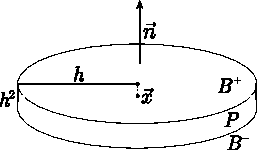
\includegraphics[width=0.6\textwidth]{images/sample.pdf}
% % \caption[caption za v kazalo]{Dolg caption pod sliko}
%   \caption[Primer vektorske slike.]{Primer vektorske slike z oznakami v enaki pisavi, kot jo
%      uporablja \LaTeX{}.  Narejena je s programom Inkscape, \LaTeX{} oznake so importane v
%      Inkscape iz pomožnega PDF.}
%   \label{fig:sample}
% \end{figure}
%
% \begin{figure}[h]
%   \centering
%   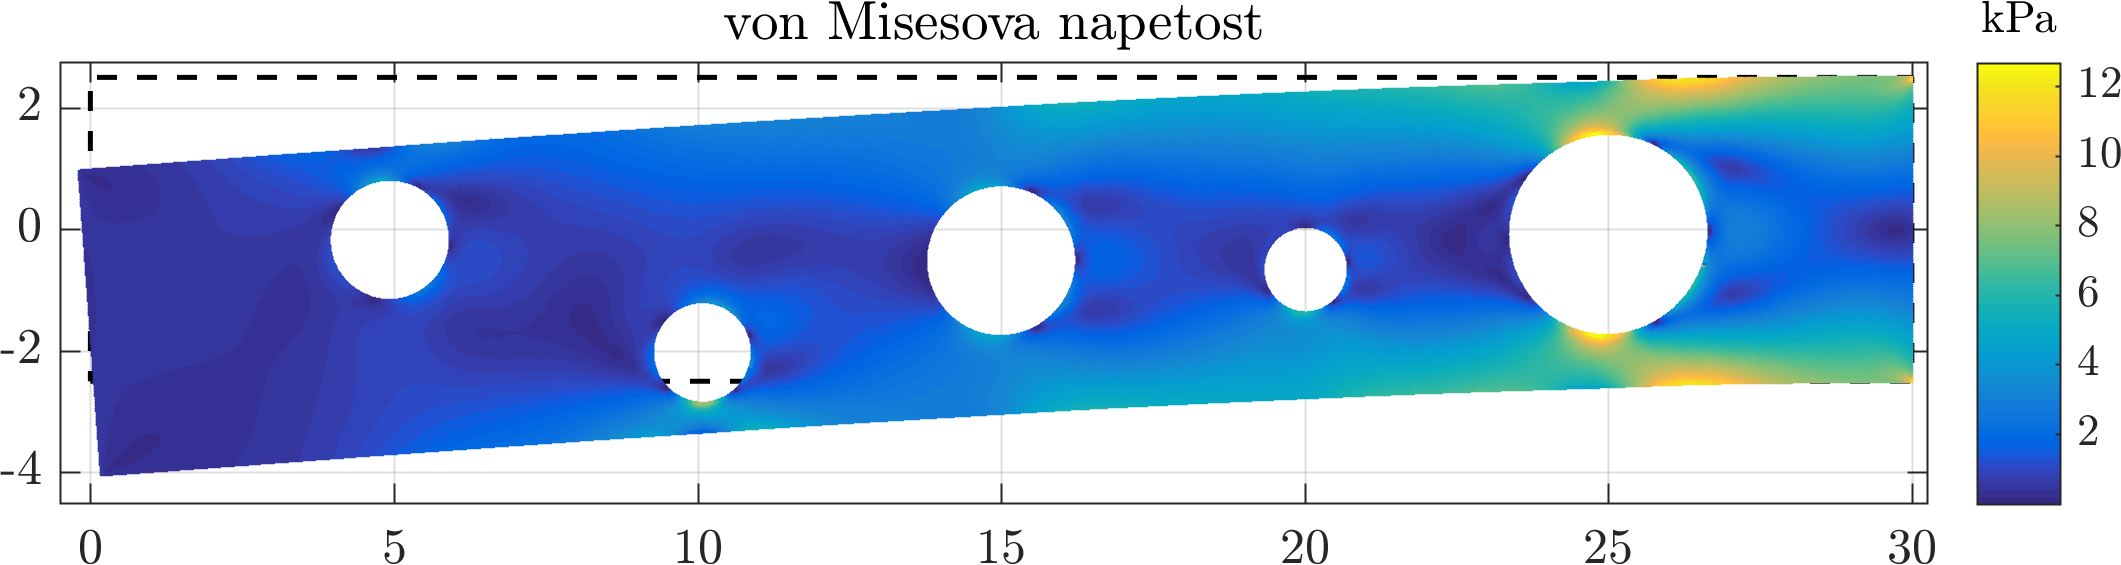
\includegraphics[width=0.8\textwidth]{images/image.png}
%   \caption[Primer bitne slike.]{Primer bitne slike, izvožene iz Matlaba. Poskrbite, da so slike v
%   dovolj visoki resoluciji in da ne vsebujejo prosojnih elementov (to zahteva PDF/A-1b format).}
%   \label{fig:image}
% \end{figure}
%
% \subsection{Kako narediti stvarno kazalo}
% Dodate ukaze \verb|\index{polje}| na besede, kjer je pojavijo, kot tukaj\index{tukaj}.
% Več o stvarnih kazalih je na voljo na \url{https://en.wikibooks.org/wiki/LaTeX/Indexing}.
%
% \subsection{Navajanje literature}
% Članke citiramo z uporabo \verb|\cite{label}|, \verb|\cite[text]{label}| ali pa več naenkrat s
% \verb|\cite\{label1, label2}|. Tudi tukaj predhodno besedo in citat povežemo z nedeljivim presledkom
% $\sim$. Na primer~\cite{chen2006meshless,liu2001point}, ali pa \cite{kibriya2007empirical}, ali pa
% \cite[str.\ 12]{trobec2015parallel}, \cite[enačba (2.3)]{pereira2016convergence}.
% Vnosi iz \verb|.bib| datoteke, ki niso citirani, se ne prikažejo v seznamu literature, zato jih
% tukaj citiram.~\cite{vene2000categorical}, \cite{gregoric2017stopniceni}, \cite{slak2015induktivni},
% \cite{nsphere}, \cite{kearsley1975linearly}, \cite{STtemplate}, \cite{NunbergerTand}, \cite{vanoosten2008realizability}.

\end{document}
